%%%%%%%%%%%%%%%%%%%%%%%%%%%%%%%%%%%%%%%%%
% The Legrand Orange Book
% LaTeX Template
% Version 1.4 (12/4/14)
%
% Important note:
% Chapter heading images should have a 2:1 width:height ratio,
% e.g. 920px width and 460px height.
%
%%%%%%%%%%%%%%%%%%%%%%%%%%%%%%%%%%%%%%%%%

%----------------------------------------------------------------------------------------
%	PACKAGES AND OTHER DOCUMENT CONFIGURATIONS
%----------------------------------------------------------------------------------------

\documentclass[11pt,openany]{book} % Default font size and left-justified equations

\usepackage{mathtools}  % for DeclareMathOperator, DeclarePairedDelimiter

\usepackage[top=3cm,bottom=3cm,left=3.2cm,right=3.2cm,headsep=10pt,a4paper]{geometry} % Page margins

\usepackage{xcolor} % Required for specifying colors by name
\definecolor{themecolor}{RGB}{41,85,26} % Define the theme color used for highlighting throughout the book
\definecolor{themeblue}{RGB}{41,26,85}
\usepackage[all]{xy}

\usepackage{hyperref}
\usepackage{enumitem}

% Font Settings
\usepackage{avant} % Use the Avantgarde font for headings
%\usepackage{times} % Use the Times font for headings
\usepackage{mathptmx} % Use the Adobe Times Roman as the default text font together with math symbols from the Symbol, Chancery and Computer Modern fonts

\usepackage{microtype} % Slightly tweak font spacing for aesthetics
\usepackage[utf8]{inputenc} % Required for including letters with accents
\usepackage[T1]{fontenc} % Use 8-bit encoding that has 256 glyphs

% Bibliography
\usepackage[style=alphabetic,sorting=nyt,sortcites=true,autopunct=true,autolang=hyphen,hyperref=true,abbreviate=false,backref=true,backend=biber]{biblatex}
\addbibresource{bibliography.bib} % BibTeX bibliography file
\defbibheading{bibempty}{}

% Index
\usepackage{calc} % For simpler calculation - used for spacing the index letter headings correctly
\usepackage{makeidx} % Required to make an index
\makeindex % Tells LaTeX to create the files required for indexing

%----------------------------------------------------------------------------------------

%----------------------------------------------------------------------------------------
%	VARIOUS REQUIRED PACKAGES
%----------------------------------------------------------------------------------------

\usepackage{titlesec} % Allows customization of titles

\usepackage[pdftex]{graphicx} % Required for including pictures
\graphicspath{{Pictures/}} % Specifies the directory where pictures are stored

\usepackage{xy}

\usepackage{lipsum} % Inserts dummy text

\usepackage{tikz} % Required for drawing custom shapes
\usepackage{tikz-cd} % Required for snazzy commutative diagrams

\usepackage{csquotes}
\usepackage[english]{babel} % English language/hyphenation

\usepackage{enumitem} % Customize lists
\setlist{nolistsep} % Reduce spacing between bullet points and numbered lists

\usepackage{booktabs} % Required for nicer horizontal rules in tables

\usepackage{microtype} % Required for nicer spacing

\usepackage{eso-pic} % Required for specifying an image background in the title page

%----------------------------------------------------------------------------------------
%	MAIN TABLE OF CONTENTS
%----------------------------------------------------------------------------------------

\usepackage{titletoc} % Required for manipulating the table of contents

\contentsmargin{0cm} % Removes the default margin
% Chapter text styling
\titlecontents{chapter}[1.25cm] % Indentation
{\addvspace{15pt}\large\sffamily\bfseries} % Spacing and font options for chapters
{\color{themecolor!60}\contentslabel[\Large\thecontentslabel]{1.25cm}\color{themecolor}} % Chapter number
{}
{\color{themecolor!60}\normalsize\sffamily\bfseries\;\titlerule*[.5pc]{.}\;\thecontentspage} % Page number
% Section text styling
\titlecontents{section}[1.25cm] % Indentation
{\addvspace{5pt}\sffamily\bfseries} % Spacing and font options for sections
{\contentslabel[\thecontentslabel]{1.25cm}} % Section number
{}
{\sffamily\hfill\color{black}\thecontentspage} % Page number
[]
% Subsection text styling
\titlecontents{subsection}[1.25cm] % Indentation
{\addvspace{1pt}\sffamily\small} % Spacing and font options for subsections
{\contentslabel[\thecontentslabel]{1.25cm}} % Subsection number
{}
{\sffamily\;\titlerule*[.5pc]{.}\;\thecontentspage} % Page number
[]

%----------------------------------------------------------------------------------------
%	MINI TABLE OF CONTENTS IN CHAPTER HEADS
%----------------------------------------------------------------------------------------

% Section text styling
\titlecontents{lsection}[0em] % Indentation
{\footnotesize\sffamily} % Font settings
{}
{}
{}

% Subsection text styling
\titlecontents{lsubsection}[.5em] % Indentation
{\normalfont\footnotesize\sffamily} % Font settings
{}
{}
{}

%----------------------------------------------------------------------------------------
%	PAGE HEADERS
%----------------------------------------------------------------------------------------

\usepackage{fancyhdr} % Required for header and footer configuration

\pagestyle{fancy}
\renewcommand{\chaptermark}[1]{\markboth{\sffamily\normalsize\bfseries\chaptername\ \thechapter.\ #1}{}} % Chapter text font settings
\renewcommand{\sectionmark}[1]{\markright{\sffamily\normalsize\thesection\hspace{5pt}#1}{}} % Section text font settings
\fancyhf{} \fancyhead[LE,RO]{\sffamily\normalsize\thepage} % Font setting for the page number in the header
\fancyhead[LO]{\rightmark} % Print the nearest section name on the left side of odd pages
\fancyhead[RE]{\leftmark} % Print the current chapter name on the right side of even pages
\renewcommand{\headrulewidth}{0.5pt} % Width of the rule under the header
\addtolength{\headheight}{2.5pt} % Increase the spacing around the header slightly
\renewcommand{\footrulewidth}{0pt} % Removes the rule in the footer
\fancypagestyle{plain}{\fancyhead{}\renewcommand{\headrulewidth}{0pt}} % Style for when a plain pagestyle is specified

% Removes the header from odd empty pages at the end of chapters
\makeatletter
\renewcommand{\cleardoublepage}{
\clearpage\ifodd\c@page\else
\hbox{}
\vspace*{\fill}
\thispagestyle{empty}
\newpage
\fi}

%----------------------------------------------------------------------------------------
%	THEOREM STYLES
%----------------------------------------------------------------------------------------

\usepackage{amsmath,amsfonts,amssymb,amsthm} % For math equations, theorems, symbols, etc

\newcommand{\intoo}[2]{\mathopen{]}#1\,;#2\mathclose{[}}
\newcommand{\ud}{\mathop{\mathrm{{}d}}\mathopen{}}
\newcommand{\intff}[2]{\mathopen{[}#1\,;#2\mathclose{]}}
\newtheorem{notation}{Notation}[chapter]

%%%%%%%%%%%%%%%%%%%%%%%%%%%%%%%%%%%%%%%%%%%%%%%%%%%%%%%%%%%%%%%%%%%%%%%%%%%
%%%%%%%%%%%%%%%%%%%% dedicated to boxed/framed environements %%%%%%%%%%%%%%
%%%%%%%%%%%%%%%%%%%%%%%%%%%%%%%%%%%%%%%%%%%%%%%%%%%%%%%%%%%%%%%%%%%%%%%%%%%
\newtheoremstyle{themecolornumbox}% % Theorem style name
{0pt}% Space above
{0pt}% Space below
{\normalfont}% % Body font
{}% Indent amount
{\small\bf\sffamily\color{themecolor}}% % Theorem head font
{\;}% Punctuation after theorem head
{0.25em}% Space after theorem head
{\small\sffamily\color{themecolor}\thmname{#1}\nobreakspace\thmnumber{\@ifnotempty{#1}{}\@upn{#2}.}% Theorem text (e.g. Theorem 2.1)
\thmnote{\nobreakspace\the\thm@notefont\sffamily\bfseries\color{black}---\nobreakspace#3.}} % Optional theorem note
\renewcommand{\qedsymbol}{$\blacksquare$}% Optional qed square

\newtheoremstyle{themecolornonumbox}% % Theorem style name
{0pt}% Space above
{0pt}% Space below
{\normalfont}% % Body font
{}% Indent amount
{\small\bf\sffamily\color{themecolor}}% % Theorem head font
{\;}% Punctuation after theorem head
{0.25em}% Space after theorem head
{\small\sffamily\color{themecolor}\thmname{#1}% Theorem text (e.g. Theorem 2.1)
\thmnote{\nobreakspace\the\thm@notefont\sffamily\bfseries\color{black}---\nobreakspace#3.}} % Optional theorem note
\renewcommand{\qedsymbol}{$\blacksquare$}% Optional qed square

\newtheoremstyle{themecolorbox}% % Theorem style name
{0pt}% Space above
{0pt}% Space below
{\normalfont}% % Body font
{}% Indent amount
{\small\bf\sffamily\color{themecolor}}% % Theorem head font
{\;}% Punctuation after theorem head
{0.25em}% Space after theorem head
{\small\sffamily\color{themecolor}\thmname{#1}% Theorem text (e.g. Theorem 2.1)
\thmnote{\nobreakspace\the\thm@notefont \bfseries #3.}} % Optional theorem note
\renewcommand{\qedsymbol}{$blacksquare$}% Optional qed square

\newtheoremstyle{blacknumex}% Theorem style name
{5pt}% Space above
{5pt}% Space below
{\normalfont}% Body font
{} % Indent amount
{\small\bf\sffamily}% Theorem head font
{\;}% Punctuation after theorem head
{0.25em}% Space after theorem head
{\small\sffamily{\tiny\ensuremath{\blacksquare}}\nobreakspace\thmname{#1}\nobreakspace\thmnumber{\@ifnotempty{#1}{}\@upn{#2}}% Theorem text (e.g. Theorem 2.1)
\thmnote{\nobreakspace\the\thm@notefont\sffamily\bfseries---\nobreakspace#3.}}% Optional theorem note

\newtheoremstyle{blacknumbox} % Theorem style name
{0pt}% Space above
{0pt}% Space below
{\normalfont}% Body font
{}% Indent amount
{\small\bf\sffamily}% Theorem head font
{\;}% Punctuation after theorem head
{0.25em}% Space after theorem head
{\small\sffamily\thmname{#1}% Theorem text (e.g. Theorem 2.1)
\thmnote{\nobreakspace\the\thm@notefont\sffamily\bfseries---\nobreakspace#3.}}% Optional theorem note

%%%%%%%%%%%%%%%%%%%%%%%%%%%%%%%%%%%%%%%%%%%%%%%%%%%%%%%%%%%%%%%%%%%%%%%%%%%
%%%%%%%%%%%%% dedicated to non-boxed/non-framed environements %%%%%%%%%%%%%
%%%%%%%%%%%%%%%%%%%%%%%%%%%%%%%%%%%%%%%%%%%%%%%%%%%%%%%%%%%%%%%%%%%%%%%%%%%
\newtheoremstyle{themecolornum}% % Theorem style name
{5pt}% Space above
{5pt}% Space below
{\normalfont}% % Body font
{}% Indent amount
{\small\bf\sffamily\color{themecolor}}% % Theorem head font
{\;}% Punctuation after theorem head
{0.25em}% Space after theorem head
{\small\sffamily\color{themecolor}\thmname{#1}\nobreakspace\thmnumber{\@ifnotempty{#1}{}\@upn{#2}}% Theorem text (e.g. Theorem 2.1)
\thmnote{\nobreakspace\the\thm@notefont\sffamily\bfseries\color{black}---\nobreakspace#3.}} % Optional theorem note
\renewcommand{\qedsymbol}{$\blacksquare$}% Optional qed square
\makeatother

% Defines the theorem text style for each type of theorem to one of the three styles above
\newcounter{dummy}
\numberwithin{dummy}{section}

\theoremstyle{themecolornumbox}
\newtheorem{theoremeT}[dummy]{Theorem}
\newtheorem{problem}{Problem}[chapter]
%\newtheorem{exerciseT}{Exercise}[chapter]
%\newtheorem{exerciseT}{Exercise}

%\theoremstyle{themecolornonumbox}
%\newtheorem{solutionT}{Solution}
\newcommand{\solutionpreskip}{-0.25em} % move closer to exercise block
\newcommand{\solutionpostskip}{0pt}
\newenvironment{solutionT}[1][]{%
\vspace{\solutionpreskip}%
  \begin{proof}[\small\bf\sffamily%
    {\color{themecolor}Solution}%
    {\ifx\relax#1\relax\else\ (#1)\fi}%
    \color{themecolor}% for the trailing period
    ]%
}{\vspace{\solutionpostskip}\end{proof}}

\theoremstyle{themecolornumbox}
\newtheorem{lemma}{Lemma}
\theoremstyle{themecolornonumbox}
\newtheorem*{lemma*}{Lemma}

\theoremstyle{themecolorbox}
\newtheorem{exerciseT}{Exercise}

\theoremstyle{blacknumex}
\newtheorem{exampleT}{Example}[chapter]

\theoremstyle{blacknumbox}
\newtheorem{vocabulary}{Vocabulary}[chapter]
\newtheorem{definitionT}{Definition}
\newtheorem{corollaryT}[dummy]{Corollary}

\theoremstyle{themecolornum}
\newtheorem{proposition}[dummy]{Proposition}
\newtheorem{claim}[dummy]{Claim}

%----------------------------------------------------------------------------------------
%	DEFINITION OF COLORED BOXES
%----------------------------------------------------------------------------------------

\RequirePackage[framemethod=default]{mdframed} % Required for creating the theorem, definition, exercise and corollary boxes

% Theorem box
\newmdenv[skipabove=7pt,
skipbelow=7pt,
backgroundcolor=black!5,
linecolor=themecolor,
innerleftmargin=5pt,
innerrightmargin=5pt,
innertopmargin=5pt,
leftmargin=0cm,
rightmargin=0cm,
innerbottommargin=5pt]{tBox}

% Exercise box	
\newmdenv[skipabove=7pt,
skipbelow=7pt,
rightline=false,
leftline=true,
topline=false,
bottomline=false,
backgroundcolor=themecolor!10,
linecolor=themecolor,
innerleftmargin=5pt,
innerrightmargin=5pt,
innertopmargin=5pt,
innerbottommargin=5pt,
leftmargin=0cm,
rightmargin=0cm,
linewidth=4pt]{eBox}	

% Definition box
\newmdenv[skipabove=7pt,
skipbelow=7pt,
rightline=false,
leftline=true,
topline=false,
bottomline=false,
linecolor=themecolor,
innerleftmargin=5pt,
innerrightmargin=5pt,
innertopmargin=0pt,
leftmargin=0cm,
rightmargin=0cm,
linewidth=4pt,
innerbottommargin=0pt]{dBox}	

% Corollary box
\newmdenv[skipabove=7pt,
skipbelow=7pt,
rightline=false,
leftline=true,
topline=false,
bottomline=false,
linecolor=gray,
backgroundcolor=black!5,
innerleftmargin=5pt,
innerrightmargin=5pt,
innertopmargin=5pt,
leftmargin=0cm,
rightmargin=0cm,
linewidth=4pt,
innerbottommargin=5pt]{cBox}

% Creates an environment for each type of theorem and assigns it a theorem text style from the "Theorem Styles" section above and a colored box from above
\newenvironment{theorem}{\begin{tBox}\begin{theoremeT}}{\end{theoremeT}\end{tBox}}
%\newenvironment{exercise}{\begin{eBox}\begin{exerciseT}}{\hfill{\color{themecolor}\tiny\ensuremath{\blacksquare}}\end{exerciseT}\end{eBox}}
\newenvironment{exercise}{\begin{eBox}\begin{exerciseT}}{\hfill{\color{themecolor}}\end{exerciseT}\end{eBox}}
% solutionT is already a proof environment; just alias it
\newenvironment{solution}[1][]{\begin{solutionT}[#1]}{\end{solutionT}}
%\hfill{\tiny\ensuremath{\blacksquare}}\end{solutionT}} \newenvironment{definition}{\begin{dBox}\begin{definitionT}}{\end{definitionT}\end{dBox}}	
\newenvironment{example}{\begin{exampleT}}{\hfill{\tiny\ensuremath{\blacksquare}}\end{exampleT}}		
\newenvironment{corollary}{\begin{cBox}\begin{corollaryT}}{\end{corollaryT}\end{cBox}}	

\newenvironment{definition}{\begin{dBox}\begin{definitionT}}{\end{definitionT}\end{dBox}}	

%----------------------------------------------------------------------------------------
%	REMARK ENVIRONMENT
%----------------------------------------------------------------------------------------

\newenvironment{remark}{\par\vspace{10pt}\small % Vertical white space above the remark and smaller font size
\begin{list}{}{
\leftmargin=35pt % Indentation on the left
\rightmargin=25pt}\item\ignorespaces % Indentation on the right
\makebox[-2.5pt]{\begin{tikzpicture}[overlay]
\node[draw=themecolor!60,line width=1pt,circle,fill=themecolor!25,font=\sffamily\bfseries,inner sep=2pt,outer sep=0pt] at (-15pt,0pt){\textcolor{themecolor}{R}};\end{tikzpicture}} % Orange R in a circle
\advance\baselineskip -1pt}{\end{list}\vskip5pt} % Tighter line spacing and white space after remark

\newenvironment{todo}{\par\vspace{10pt}\small % Vertical white space above the todo and smaller font size
\begin{list}{}{
\leftmargin=35pt % Indentation on the left
\rightmargin=25pt}\item\ignorespaces % Indentation on the right
\makebox[-2.5pt]{\begin{tikzpicture}[overlay]
\node[draw=themeblue!60,line width=1pt,circle,fill=themeblue!25,font=\sffamily\bfseries,inner sep=2pt,outer sep=0pt] at (-15pt,0pt){\textcolor{themeblue}{P}};\end{tikzpicture}} % Blue P (pending) in a circle
\advance\baselineskip -1pt}{\end{list}\vskip5pt} % Tighter line spacing and white space after remark


%----------------------------------------------------------------------------------------
%	SECTION NUMBERING IN THE MARGIN
%----------------------------------------------------------------------------------------

\makeatletter
\renewcommand{\@seccntformat}[1]{\llap{\textcolor{themecolor}{\csname the#1\endcsname}\hspace{1em}}}
\renewcommand{\section}{\@startsection{section}{1}{\z@}
{-4ex \@plus -1ex \@minus -.4ex}
{1ex \@plus.2ex }
{\normalfont\large\sffamily\bfseries}}
\renewcommand{\subsection}{\@startsection {subsection}{2}{\z@}
{-3ex \@plus -0.1ex \@minus -.4ex}
{0.5ex \@plus.2ex }
{\normalfont\sffamily\bfseries}}
\renewcommand{\subsubsection}{\@startsection {subsubsection}{3}{\z@}
{-2ex \@plus -0.1ex \@minus -.2ex}
{.2ex \@plus.2ex }
{\normalfont\small\sffamily\bfseries}}
\renewcommand\paragraph{\@startsection{paragraph}{4}{\z@}
{-2ex \@plus-.2ex \@minus .2ex}
{.1ex}
{\normalfont\small\sffamily\bfseries}}

%----------------------------------------------------------------------------------------
%	HYPERLINKS IN THE DOCUMENTS
%----------------------------------------------------------------------------------------

% For an unclear reason, the package should be loaded now and not later
\usepackage{hyperref}
\hypersetup{hidelinks,colorlinks=false,breaklinks=true,urlcolor= themecolor,bookmarksopen=false,pdftitle={Title},pdfauthor={Author}}
\usepackage[noabbrev]{cleveref}

%----------------------------------------------------------------------------------------
%	CHAPTER HEADINGS
%----------------------------------------------------------------------------------------

% The set-up below should be (sadly) manually adapted to the overall margin page septup controlled by the geometry package loaded in the main.tex document. It is possible to implement below the dimensions used in the geometry package (top,bottom,left,right)... TO BE DONE

\newcommand{\thechapterimage}{}
\newcommand{\chapterimage}[1]{\renewcommand{\thechapterimage}{#1}}

% Numbered chapters with mini tableofcontents
\def\thechapter{\arabic{chapter}}
\def\@makechapterhead#1{
\thispagestyle{empty}
{\centering \normalfont\sffamily
\ifnum \c@secnumdepth >\m@ne
\if@mainmatter
\startcontents
\begin{tikzpicture}[remember picture,overlay]
\node at (current page.north west)
{\begin{tikzpicture}[remember picture,overlay]
\node[anchor=north west,inner sep=0pt] at (0,0) %{\ifx\relax\thechapterimage\relax\includegraphics[width=\paperwidth]{\thechapterimage}\fi};
{};
%%%%%%%%%%%%%%%%%%%%%%%%%%%%%%%%%%%%%%%%%%%%%%%%%%%%%%%%%%%%%%%%%%%%%%%%%%%%%%%%%%%%%
% Commenting the 3 lines below removes the small contents box in the chapter heading
%\fill[color=themecolor!10!white,opacity=.6] (1cm,0) rectangle (8cm,-7cm);
%\node[anchor=north west] at (1.1cm,.35cm) {\parbox[t][8cm][t]{6.5cm}{\huge\bfseries\flushleft \printcontents{l}{1}{\setcounter{tocdepth}{2}}}};
\draw[anchor=west] (2cm,-2.5cm) node [rounded corners=20pt,fill=themecolor!10!white,text opacity=1,draw=themecolor,draw opacity=1,line width=1.5pt,fill opacity=.6,inner sep=12pt]{\huge\sffamily\bfseries\textcolor{black}{\thechapter. #1\strut\makebox[22cm]{}}};
%%%%%%%%%%%%%%%%%%%%%%%%%%%%%%%%%%%%%%%%%%%%%%%%%%%%%%%%%%%%%%%%%%%%%%%%%%%%%%%%%%%%%
\end{tikzpicture}};
\end{tikzpicture}}
\par\vspace*{20\p@}
\fi
\fi}

% Unnumbered chapters without mini tableofcontents (could be added though)
\def\@makeschapterhead#1{
\thispagestyle{empty}
{\centering \normalfont\sffamily
\ifnum \c@secnumdepth >\m@ne
\if@mainmatter
\begin{tikzpicture}[remember picture,overlay]
\node at (current page.north west)
{\begin{tikzpicture}[remember picture,overlay]
\node[anchor=north west,inner sep=0pt] at (0,0) %{\includegraphics[width=\paperwidth]{\thechapterimage}}; % Remove comment (and comment out next line) to include chapter heading image
{}; % Adjust anchor coordinates below to move chapter heading
\draw[anchor=west] (2cm,-3cm) node [rounded corners=20pt,fill=themecolor!10!white,fill opacity=.6,inner sep=12pt,text opacity=1,draw=themecolor,draw opacity=1,line width=1.5pt]{\huge\sffamily\bfseries\textcolor{black}{#1\strut\makebox[22cm]{}}};
\end{tikzpicture}};
\end{tikzpicture}}
\par\vspace*{50\p@} % Adjust spacing below chapter heading
\fi
\fi
}
\makeatother % Insert the commands.tex file which contains the majority of the structure behind the template

\setlength{\parindent}{0in} % Removes the indenting at the start of each paragraph

%----------------------------------------------------------------------------------------
%	Useful Commands
%----------------------------------------------------------------------------------------

% natural transformation (\tau : S \naturalto T)
% adapated from http://tex.stackexchange.com/a/141018/37357
\DeclareRobustCommand{\naturalto}{%
  \mathrel{\vbox{\offinterlineskip
    \mathsurround=0pt
    \ialign{\hfil##\hfil\cr
      \!\normalfont\scalebox{1.2}{.}\cr
      $\rightarrow$\cr}
  }}%
}

\newcommand{\R}{\mathbf{R}}
\newcommand{\Z}{\mathbf{Z}}
\newcommand{\Q}{\mathbf{Q}}
\newcommand{\C}{\mathbf{C}}
\newcommand{\spc}{\operatorname{Spec}}
\newcommand{\Tr}{\operatorname{Tr}}
\newcommand{\Aut}{\operatorname{Aut}}
\newcommand{\Mor}{\operatorname{Mor}}
\newcommand{\Coprod}{\rotatebox[origin=c]{180}{$\prod$}}
\newcommand{\xsets}[1]{#1\textnormal{-}\mathbf{sets}}
\newcommand{\coker}{\operatorname{coker}}

\let\amalg=\undefined
\let\coprod=\undefined
\DeclareSymbolFont{cmsymbols}{OMS}{cmsy}{m}{n}
\DeclareSymbolFont{cmlargesymbols}{OMX}{cmex}{m}{n}
\DeclareMathSymbol{\amalg}{\mathbin}{cmsymbols}{"71}
\DeclareMathSymbol{\coprod}{\mathop}{cmlargesymbols}{"60}
%\renewcommand{\thesection}{\arabic{section}} % Remove chapter number from numbering

%----------------------------------------------------------------------------------------

%%%%%%%%%%%%%%%%%%

% Fancy Quoting

\definecolor{quotemark}{gray}{0.7}
\makeatletter
\def\fquote{%
    \@ifnextchar[{\fquote@i}{\fquote@i[]}%]
           }%
\def\fquote@i[#1]{%
    \def\tempa{#1}%
    \@ifnextchar[{\fquote@ii}{\fquote@ii[]}%]
                 }%
\def\fquote@ii[#1]{%
    \def\tempb{#1}%
    \@ifnextchar[{\fquote@iii}{\fquote@iii[]}%]
                      }%
\def\fquote@iii[#1]{%
    \def\tempc{#1}%
    \vspace{1em}%
    \noindent%
    \begin{list}{}{%
         \setlength{\leftmargin}{0.1\textwidth}%
         \setlength{\rightmargin}{0.1\textwidth}%
                  }%
         \item[]%
         \begin{picture}(0,0)%
         \put(-15,-5){\makebox(0,0){\scalebox{3}{\textcolor{quotemark}{``}}}}%
         \end{picture}%
         \begingroup\itshape}%
 %%%%********************************************************************
 \def\endfquote{%
 \endgroup\par%
 \makebox[0pt][l]{%
 \hspace{0.8\textwidth}%
 \begin{picture}(0,0)(0,0)%
 \put(15,15){\makebox(0,0){%
 \scalebox{3}{\color{quotemark}''}}}%
 \end{picture}}%
 \ifx\tempa\empty%
 \else%
    \ifx\tempc\empty%
       \hfill\rule{100pt}{0.5pt}\\\mbox{}\hfill\tempa,\ \tempb%
   \else%
       \hfill\rule{100pt}{0.5pt}\\\mbox{}\hfill\tempa,\ \tempb,\ \tempc%
   \fi\fi\par%
   \vspace{0.5em}%
 \end{list}%
 }%
 \makeatother

%----------------------------------------------------------------------------------------

\begin{document}

%----------------------------------------------------------------------------------------
%----------------------------------------------------------------------------------------
%----------------------------------------------------------------------------------------
%	TITLE PAGE
%----------------------------------------------------------------------------------------
%----------------------------------------------------------------------------------------
%----------------------------------------------------------------------------------------

\begingroup
\thispagestyle{empty}
%\AddToShipoutPicture*{\put(6,5){\includegraphics[scale=1]{background}}} % Image background
\centering
\vspace*{9cm}
\par\normalfont\fontsize{35}{35}\sffamily\selectfont
{Grothendieck's Galois Theory: From Fields to Schemes}\par % Book title
\vspace*{1cm}
{\Huge Nolan Schock}\par % Author name
\endgroup

%----------------------------------------------------------------------------------------
%	APPROVAL PAGE
%----------------------------------------------------------------------------------------

\newpage
%~\vfill
\thispagestyle{empty}

\begin{center}
{\Large APPROVAL PAGE}
\end{center}

\vspace{2in}
\noindent {\sc TITLE:} {Grothendieck's Galois Theory: From Fields to Schemes}

\vspace{0.25in}
\noindent {\sc AUTHOR:} Nolan Schock

\vspace{0.25in}
\noindent {\sc DATE SUBMITTED:}

\vspace{3in}
\begin{minipage}{0.5\textwidth}
\underline{\hspace{2.5in}}

\noindent Senior Project Advisor
\end{minipage}
\begin{minipage}{0.5\textwidth}
\underline{\hspace{2.5in}}

\noindent Signature
\end{minipage}

\vspace{1in}
\begin{minipage}{0.5\textwidth}
\underline{\hspace{2.5in}}

\noindent Mathematics Department Chair
\end{minipage}
\begin{minipage}{0.5\textwidth}
\underline{\hspace{2.5in}}

\noindent Signature
\end{minipage}

%----------------------------------------------------------------------------------------
%----------------------------------------------------------------------------------------
%----------------------------------------------------------------------------------------
%	TABLE OF CONTENTS
%----------------------------------------------------------------------------------------
%----------------------------------------------------------------------------------------
%----------------------------------------------------------------------------------------

%\chapterimage{chapter_head_1.pdf} % Table of contents heading image
%
%\pagestyle{empty} % No headers
%
\tableofcontents % Print the table of contents itself
%
%\cleardoublepage % Forces the first chapter to start on an odd page so it's on the right
%
%\pagestyle{fancy} % Print headers again

%----------------------------------------------------------------------------------------
%----------------------------------------------------------------------------------------
%----------------------------------------------------------------------------------------
%	CHAPTER - Introduction
%----------------------------------------------------------------------------------------
%----------------------------------------------------------------------------------------
%----------------------------------------------------------------------------------------

\chapter{Introduction}

Alexander Grothendieck once poetically explained his abstract approach to mathematics through the following metaphor.\\

\begin{fquote}[Alexander Grothendieck][\cite{grothendieck}]
I can illustrate the ... approach with the ... image of a nut to be opened. The first analogy that came to my mind is of immersing the nut in some softening liquid, and why not simply water? From time to time you rub so the liquid penetrates better, and otherwise you let time pass. The shell becomes more flexible through weeks and months — when the time is ripe, hand pressure is enough, the shell opens like a perfectly ripened avocado! ...\\

The unknown thing to be known appeared to me as some stretch of earth or hard marl, resisting penetration… the sea advances insensibly in silence, nothing seems to happen, nothing moves, the water is so far off you hardly hear it.. yet it finally surrounds the resistant substance.
\end{fquote}

This paper takes such an abstract viewpoint to heart, diving only surface deep into the vast sea Grothendieck helped develop.\\

Of particular interest to us is the generalization of Galois theory for fields. Originally developed by Grothendieck, this generalization illuminates the geometric structure inherent in Galois theory, strongly linking the fundamental theorem of Galois theory with the classification of covering spaces of a topological space. The generalization goes even farther, giving an analogous classification of finite \'etale coverings of schemes, and defining algebraic and geometric analogues of the topological fundamental group. This is the start of a deep and actively studied topic of research, linking fundamental topological properties of curves and surfaces to heavily algebraic notions. It is in such a theory that one truly sees the beauty and power of algebraic geometry.\\

Before even beginning to dive into generalizations of Galois theory, we must discuss several preliminary ideas. In Chapter \ref{prelim} we quickly review the basic notions from category theory, algebra, and topology which will be crucial to us. We then spend Chapter \ref{sheaves} explaining in detail the notion of a sheaf in preparation for Chapter \ref{schemes}, where we give a brief and incomplete overview of the true objects of our affections and the focal point of Grothendieck's theory of algebraic geometry: schemes. We conclude in Chapter \ref{galois} by finally describing Galois theory in its most general glory.\\

The nature of this paper is such that we must leave out many important details for the sake of brevity and an attempt at clean exposition. The reader will find many theorems and few proofs; additionally our exposition of scheme theory is woefully incomplete, developing only the necessary background for our description of Galois theory. The interested reader is encouraged to find more detail in \cite{vakil}, \cite{hartshorne}, and the original sources of \cite{grothendieckega} and \cite{grothendiecksga}.
%----------------------------------------------------------------------------------------
%----------------------------------------------------------------------------------------
%----------------------------------------------------------------------------------------
%	CHAPTER - Preliminaries
%----------------------------------------------------------------------------------------
%----------------------------------------------------------------------------------------
%----------------------------------------------------------------------------------------

\chapter{Preliminaries} \label{prelim}
In this chapter we rapidly develop the necessary notions from category theory, algebra, and topology. 

\section{Conventions}
All rings are supposed commutative with unity.\\

We denote by $\mathbf{Sets}$ the category of sets, $\mathbf{sets}$ the category of finite sets, $\mathbf{Grp}$ the category of groups, $\mathbf{Ab}$ the category of abelian groups, $\mathbf{Rng}$ the category of rings, $\mathbf{Mod}_R$ the category of modules over a ring $R$, $\mathbf{Alg}_R$ the category of algebras over a ring $R$, $\mathbf{Top}$ the category of topological spaces, and $\mathbf{Top}_*$ the category of pointed topological spaces.\\

If $A,B$ are two objects in a category $\mathcal{C}$, we write $A,B \in \mathcal{C}$, and denote by $\Mor(A,B)$ the set of morphisms from $A$ to $B$.

%----------------------------------------------------------------------------------------
%----------------------------------------------------------------------------------------
%----------------------------------------------------------------------------------------

\section{Category Theory}
We assume working familiarity with the basic notions of category theory, including limits, colimits, universal properties, and adjoint functors. For additional information on these and other notions, we refer the reader to \cite{maclane}. This section will give a minimal amount of additional background needed for our purposes, and establish some terminology.\\


\begin{definition}
A category $\mathcal{C}$ is \emph{equivalent} to a category $\mathcal{D}$ if there is a pair of functors $F : \mathcal{C} \to \mathcal{D}$ and $G : \mathcal{D} \to \mathcal{C}$ such that $GF$ is isomorphic to $\operatorname{id}_{\mathcal{C}}$ and $FG$ is isomorphic to $\operatorname{id}_{\mathcal{D}}$.\\

Two categories $\mathcal{C}$ and $\mathcal{D}$ are said to be \emph{anti-equivalent} if $\mathcal{C}$ is equivalent to the opposite category $\mathcal{D}^{op}$. (Or equivalently, $\mathcal{C}^{op}$ is equivalent to $\mathcal{D}$.)
\end{definition}

\begin{definition}
\item A category $\mathcal{C}$ is said to be \emph{additive} if it satisfies the following properties:
\begin{enumerate}
	\item For each $A,B \in \mathcal{C}$, $\Mor(A,B)$ is an abelian group such that composition of morphisms distributes over addition.
    \item The category $\mathcal{C}$ has a zero object, denoted $0$.
    \item Finite products exist in $\mathcal{C}$.
\end{enumerate}

In an additive category, morphisms are often called \emph{homomorphisms}, and $\Mor(A,B)$ is often labeled $\operatorname{Hom}(A,B)$.\\

\item A category $\mathcal{C}$ is said to be \emph{abelian} if it is additive and additionally satisfies the following properties:
\begin{enumerate}
	\item Every morphism has a kernel and a cokernel.
    \item Every monomorphism is the kernel of its cokernel.
    \item Every epimorphism is the cokernel of its kernel.
\end{enumerate}
\end{definition}

\begin{example}\
	\begin{itemize}
	\item $\mathbf{sets}$ and $\mathbf{Grp}$ are additive categories.
	\item $\mathbf{Ab}$ and $\mathbf{Mod}_R$ are abelian categories.
    \end{itemize}
We will later see that sheaves of abelian groups form an abelian category.
\end{example}

\begin{definition}
Let $\mathcal{C}$ be an abelian category. A sequence
\[
\cdots \rightarrow A \xrightarrow{f} B \xrightarrow{g} C \rightarrow \cdots
\]
in $\mathcal{C}$ is \emph{exact at $B$} if $\operatorname{ker} g = \operatorname{im} f$. A sequence is \emph{exact} if it is exact at each object.

A functor $F$ is \emph{right-exact} if exactness of
\[
A \to B \to C \to 0
\]
implies exactness of
\[
F(A) \to F(B) \to F(C) \to 0,
\]
and \emph{left-exact} if exactness of 
\[
0 \to A \to B \to C
\]
implies exactness of
\[
0 \to F(A) \to F(B) \to F(C).
\]
A functor $F$ is \emph{exact} if it is both left-exact and right-exact.
\end{definition}

A particularly important instance of a categorical limit is a projective limit. We will use this notion essentially in our development of generalizations of Galois theory.\\

\begin{definition}
Let $\mathcal{I}$ be a directed, partially ordered category. A diagram in a category $\mathcal{C}$ indexed by $\mathcal{I}$ is called a \emph{projective system}. The limit of a projective system is called a \emph{projective limit}, and is denoted $\varprojlim_{\pi_i \in \mathcal{I}} \pi_i$.
\end{definition}

Concretely, if the objects of $\mathcal{C}$ look like sets $\pi_i$ and the morphisms are $(f_{ij} : \pi_i \to \pi_j)_{i,j \in \mathcal{I}, i \geq j}$, then the projective limit looks like
\[
\varprojlim \pi_i = \left\{(x_i)_{i \in \mathcal{I}} \in \prod_{i \in \mathcal{I}} \pi_i \mid f_{ij}(x_i) = x_j \text{ for all } i,j \in \mathcal{I} \text{ with } i \geq j\right\}.
\]

The notions of representable and pro-representable functors are quite important, although we do not use them often in this paper\footnote{In fact, we only reference pro-representable functors in one theorem, which could probably be rephrased to remove the reference. No turning back now.}. We state them here anyway, following closely the treatment of \cite{szamuely}.\\

\begin{definition}
Let $\mathcal{C}$ be a category. A functor $F : \mathcal{C} \to \mathbf{Sets}$ is \emph{representable} if there is an object $C \in \mathcal{C}$ and an isomorphism of functors $F \simeq \operatorname{Mor}(C,-)$. The object $C$ is called the \emph{representing object}.\\

A functor $F$ is \emph{pro-representable} if there is a projective system $(P_{\alpha}, \phi_{\alpha\beta})$ of objects in $\mathcal{C}$ and a functorial isomorphism
\[
F(X) \simeq \varinjlim \operatorname{Mor}(P_{\alpha},X)
\]
for each $X \in \mathcal{C}$.
\end{definition}

Observe that if $C$ and $D$ are objects in $\mathcal{C}$, then every morphism $D \to C$ induces a natural transformation $\operatorname{Mor}(C, -) \to \operatorname{Mor}(D, -)$ via composition.\\

\begin{lemma}[Yoneda]
If $F$ and $G$ are functors $\mathcal{C} \to \mathbf{Sets}$ represented by objects $C$ and $D$, respectively, then every natural transformation $\Phi : F \to G$ is induced by a unique morphism $D \to C$.
\end{lemma}

%----------------------------------------------------------------------------------------
%----------------------------------------------------------------------------------------
%----------------------------------------------------------------------------------------

\section{Topology}

Basic knowledge of topology and algebraic topology is assumed. For more information, see \cite{munkres} and \cite{massey}.

%----------------------------------------------------------------------------------------
%----------------------------------------------------------------------------------------

\subsection{Covering Spaces}
\begin{definition}
Let $p : X \to Y$ be a continuous, surjective map of topological spaces. If every point of $Y$ has a neighborhood $U$ such that the preimage $p^{-1}(U)$ can be written as the union of disjoint open sets $V_{\alpha}$, with $p\restriction_{V_{\alpha}} : V_{\alpha} \to U$ a homeomorphism for each $V_{\alpha}$, then we say that $p$ is a \emph{covering map}, and $X$ is a \emph{covering space} for $Y$.
\end{definition}

The above definition can be reformulated in a way that will generalize more nicely for us.\\

\begin{definition}
Let $p : X \to Y$ be a continuous map of topological spaces. If $X$ can be identified as $Y \times E$ for some discrete set $E$, such that $p$ can be viewed as the projection $Y \times E \to Y$ onto the first coordinate, then $p$ is called a \emph{trivial covering}.
\end{definition}

\begin{proposition}
Let $p : X \to Y$ be a continuous map of topological spaces. Then $p$ is a covering map of $Y$ if and only if each point of $Y$ has an open neighborhood $U$ such that $p\restriction_{p^{-1}(U)} : p^{-1}(U) \to U$ is a trivial covering.
\end{proposition}
\medskip

Dual to the notion of a covering map is an \'etale map, or local homeomorphism.\\

\begin{definition}
Let $p : X \to Y$ be a continuous map of topological spaces. If every point of $X$ has an open neighborhood $U$ such that $p(U)$ is open and $p\restriction_U : U \to p(U)$ is a homeomorphism, then $p$ is said to be a \emph{local homeomorphism}, or an \emph{\'etale map}, and $X$ is said to be an \emph{\'etale space} over $Y$.
\end{definition}

Note the key difference between a covering map and an \'etale map: a covering map is local on the target, while an \'etale map is local on the source. The following proposition follows immediately from the definitions.\\

\begin{proposition}
Every covering space is \'etale.
\end{proposition}
\medskip

The converse to the above proposition does not hold, as seen in the following example.\\

\begin{example}
The map $\R^+ \to S^1$ defined by $x \mapsto e^{2\pi i x}$ is \'etale but is not a covering map.
\end{example}

Generalizing the notion of an \'etale map of topological spaces will eventually lead us to \'etale morphisms of schemes.

%----------------------------------------------------------------------------------------
%----------------------------------------------------------------------------------------

\subsection{Profinite Groups}
\begin{definition}
A \emph{topological group} is a group $G$ together with a topology on $G$, such that the group operation $G \times G \to G$, $(x,y) \mapsto xy$, and the inverse map $G \to G$, $x \mapsto -x$ are continuous.
\end{definition}

\begin{definition}
Suppose $(\pi_i)_{i \in \mathcal{I}}$ is a projective system of finite groups, where each $f_{ij} : \pi_i \to \pi_j$ is a group morphism. Then $\pi = \varprojlim \pi_i$ is a group, called a \emph{profinite group}.\\

There is an evident notion of a \emph{morphism of profinite groups}. We can therefore form a category of profinite groups.
\end{definition}

\begin{remark}
There is nothing particular to using groups in the above definition; one could similarly define profinite rings, modules, etc.
\end{remark}

\begin{lemma}
If each $\pi_i$ is endowed with the discrete topology, then the profinite group $\pi$ is a topological group. In particular, a morphism of finite groups is precisely a continuous group morphism.
\end{lemma}
\medskip

The following theorem gives an equivalent definition of a profinite group.\\

\begin{theorem} \label{profin}
A topological group is profinite if and only if it is compact and totally disconnected.
\end{theorem}

\begin{example}\
\begin{itemize}
	\item Any finite group is profinite, when given the discrete topology. Specifically, it is the projective limit of the boring diagram consisting only of itself.

	\item Let $p$ be a prime number. The $p$-adic integers $\Z_p$ are the profinite ring arising as the projective limit in the following diagram.
\[
\begin{tikzcd}
\Z_p \ar[rd] \ar[rrd] \ar[rrrd] \\
\cdots \ar[r] & \Z/p^3\Z \ar[r] & \Z/p^2\Z \ar[r] & \Z/p\Z.
\end{tikzcd}
\]

	\item Let $G$ be any group, and $\mathcal{I}$ the collection of subgroups of finite index in $G$, partially ordered by $N \geq N' \iff N \subseteq N'$. Then $(G/N)_{N \in \mathcal{I}}$ is a projective system of finite groups. The projective limit is denoted $\hat{G} = \varprojlim G/N$, and is called the \emph{profinite completion of $G$}. In particular, for $G = \Z$, we have $\hat{\Z} = \varprojlim_{n > 0} \Z/n\Z$, the group of positive integers partially ordered by divisibility. In fact, since $\Z$ is a ring, $\hat{\Z}$ is a profinite ring.
\end{itemize}
\end{example}

\medskip
If one has an action (see \ref{groupactions}) of a profinite group $\pi$ on a set $E$, which is continuous in the sense that the map $\pi \times E \to E$ is continuous when $E$ has the discrete topology and $\pi \times E$ the product topology, then $E$ is called a $\pi$-set. A morphism of $\pi$-sets is defined in the obvious way, and allows us to speak of the category of $\pi$-sets. In particular, denote the category of finite $\pi$-sets by $\pi$-$\mathbf{sets}$.

%----------------------------------------------------------------------------------------
%----------------------------------------------------------------------------------------
%----------------------------------------------------------------------------------------

\section{Algebra}

We also assume working knowledge of basic notions from algebra, including group theory, ring theory, and field theory. More information can be found in \cite{dandf}

%----------------------------------------------------------------------------------------
%----------------------------------------------------------------------------------------
\subsection{Group Actions} \label{groupactions}
We briefly review the basic notions of group actions.\\

\begin{definition}
If $G$ is a group and $E$ is an object in some category $\mathcal{C}$, then an \emph{action} of $G$ on $E$ is a group morphism $G \to \Aut_{\mathcal{C}}E$.
\end{definition}

We are usually interested in the case where $E \in \mathbf{Sets}$ or some other category where the objects are sets with additional structure. In such a case, one can view a group action as a way to permute all the elements of $E$. In particular, we have the following more specific definition.\\

\begin{definition}
A \emph{group action} of a group $G$ on a set $E$ is a set function $G \times E \to E$, written $g \cdot e$ for all $g \in G$ and $e \in E$ such that, for all $g_1,g_2 \in G$ and all $e \in E$, the following properties hold:
\begin{enumerate}
	\item $g_1 \cdot (g_2 \cdot e) = (g_1g_2) \cdot e$,
    \item $1 \cdot e = e$.
\end{enumerate}
\end{definition}

The reader can easily verify that when $\mathcal{C} = \mathbf{Sets}$, the two definitions are equivalent.\\

\begin{definition} Suppose a group $G$ acts on a set $E$. We say this action is \emph{trivial} if $g \cdot e = e$ for all $g \in G$ and all $e \in E$. The action is \emph{free} if $g \cdot e \neq e$ for all $g \in G$ and all $e \in E$.

\medskip
For an element $e \in E$, the set 
\[G\cdot e := \{g \cdot e \mid g \in G\}\]
is called the \emph{orbit} of $G$ containing $e$. The action is \emph{transitive} if it has exactly one orbit.
\end{definition}

\begin{definition}
A set $E$ together with an action of a group $G$ is called a $G$-\emph{set}. A \emph{morphism of $G$-sets} is a map $f : E \to E'$ satisfying $f(g\cdot e) = g\cdot f(e)$ for all $g \in G$ and all $e \in E$. Let $G$-$\mathbf{sets}$ denote the category of finite $G$-sets.
\end{definition}

\begin{remark}
One can generalize the notion of a morphism of $G$-sets. Suppose $E$ is a $G$-set and $E'$ is a $G'$-set, and that we have a group morphism $\varphi : G \to G'$. The natural way to define a morphism $f : E \to E'$ is to require $f(g\cdot e) = \varphi(g)\cdot f(e)$ for all $g \in G$ and all $e \in E$. Our usual notion of a morphism of $G$-sets is recovered from this in the special case where $G = G'$ and $\varphi$ is the identity map.
\end{remark}

%----------------------------------------------------------------------------------------
%----------------------------------------------------------------------------------------

\subsection{Fields}

Here we quickly establish some basic definitions from field theory necessary for our later discussion of Galois Theory. Throughout , fix a field extension $k \to L$.\\

\begin{definition}
An element $\alpha \in L$ is said to be \emph{algebraic over $k$} if it is the root of some nonzero polynomial over $k$. Among all such polynomials, there is a unique polynomial that is monic and irreducible. It is called the \emph{minimal polynomial of $\alpha$} over $k$, and denoted $m_{\alpha,k}(x)$. If all $\alpha \in L$ are algebraic over $k$, then $k\to L$ is called an \emph{algebraic extension}.
\end{definition}

\begin{definition}
If $f(x)\in k[x]$ factors completely into linear factors (\emph{splits completely}) in $L[x]$, and there is no proper intermediate extension $k \to F \to L$ such that $f(x)$ spits completely in $F[x]$, then $k\to L$ is called a \emph{splitting field extension} of $f(x)$.\\

If $L$ is an algebraic extension of $k$ such that every irreducible polynomial in $k[x]$ either splits completely or has no roots over $L$ is called \emph{normal}.\\

If $L$ is an algebraic extension of $k$ and every polynomial in $k[x]$ splits completely in $L[x]$, then $L$ is called an \emph{algebraic closure} of $k$. It is unique up to isomorphism, and is often denoted $\overline{k}$.
\end{definition}

\begin{definition}
A field $k$ is said to be \emph{algebraically closed} if every polynomial in $k[x]$ has a root in $k$.
\end{definition}

The following definition is important for us, in that we will later generalize it to algebras.

\begin{definition}
A polynomial $f(x) \in k[x]$ is said to be \emph{separable} if all of its roots (in $\overline{k}$) are distinct, and \emph{inseparable} otherwise.\\

If $k \to F$ is a field extension, then $\alpha \in F$ is said to be \emph{separable} over $k$ if $\alpha$ is algebraic and its minimal polynomial $m_{\alpha,k}(x) \in k[x]$ is separable, and \emph{inseparable} otherwise.\\

If $k \to F$ is an algebraic field extension, then $F$ is a \emph{separable extension} if every $\alpha \in F$ is separable over $k$.
\end{definition}

Denote by $\Aut_k(L)$ the group of automorphisms of $L$ that fix each element of $k$.\\

\begin{lemma} \label{galextdef}
The following are equivalent:
\begin{enumerate}
	\item The elements of $L$ fixed by $\Aut_k(L)$ are precisely those of $k$.
    \item $k \to L$ is normal and separable.
    \item $L$ is a splitting of a separable polynomial in $k$.
\end{enumerate}
\end{lemma}
\medskip

\begin{definition}
The extension $k \to L$ is said to be \emph{Galois} if any one of the conditions holds in Lemma \ref{galextdef}.
In this case, we write $\operatorname{Gal}_k(L) := \Aut_k(L)$.
\end{definition}

\begin{definition}
For an algebraic closure $\overline{k}$ of $k$, let $k_s$ be the smallest subfield of $\overline{k}$ containing each finite separable intermediate extension of $k \to \overline{k}$. Then $k_s$ is called a \emph{separable closure} of $k$. Note that $k_s$ is itself a separable, and in fact Galois, extension. We call its Galois group the \emph{absolute Galois group} of $k$.
\end{definition}

\begin{lemma}
If $k$ is a field, any Galois extension of $k$ can be embedded in a separable closure $k_s$ of $k$. Furthermore, we can identify Galois extensions $k \to L$ with sets of morphisms $\Mor_k(L, k_s)$.
\end{lemma}

%----------------------------------------------------------------------------------------
%----------------------------------------------------------------------------------------

\subsection{Modules and Algebras}

%----------------------------------------------------------------------------------------
\subsubsection{Modules}

Intuitively, a module is a ``vector space over a ring.'' In other words, a module is the action of a ring on an abelian group. More formally, we have the following definition.

\begin{definition}
Suppose $A$ is a ring and $M$ is an abelian group. Then $M$ is an \emph{$A$-module} if there is an action $A \times M \to M$ of $A$ on $M$, denoted $am$, such that, for all $a,b \in A$ and $m,n \in M$, the following hold:
\begin{enumerate}
	\item $(a+b)m = am + bm$,
    \item $(ab)m = a(bm)$,
    \item $a(m+n) = am + an$, and
    \item $1m = m$.
\end{enumerate}
\end{definition}

\begin{definition}
Let $M$ be a module over the ring $A$. A collection $(w_i)_{i \in I}$ of elements of $M$ is a \emph{basis} of $M$ if for each $x \in M$, there is a unique collection $(u_i)_{i \in I}$ of elements of $A$ such that $a_i = 0$ for all but finitely many $i \in I$, and $x = \sum_{i \in I} a_iw_i$.\\

A module which has a basis is called \emph{free}.
\end{definition}

\begin{lemma}
If $A$ is not the zero ring and $M$ is a free $A$-module with basis $(w_i)_{i \in I}$, then the cardinality $\#I$ is independent of the choice of basis.
\end{lemma}

\begin{definition}
The \emph{rank} of a free module $M$ over $A$ is the cardinality of its basis, and is denoted $\operatorname{rank}_A(M)$. If $\operatorname{rank}_A(M)$ is finite, we say that $M$ is \emph{finitely generated} as an $A$-module.
\end{definition}

\begin{example}
Let $A$ be a ring.
\begin{itemize}
	\item $A^n$ is an $A$-module of rank $n$.
    \item $A[x_1,\ldots,x_n]$ is an $A$-module of rank $n$.
    \item Any abelian group can be recognized as a $\Z$-module, and conversely any $\Z$-module can be recognized as an abelian group.
\end{itemize}
\end{example}

\begin{definition}
If $M,N$ are $A$-modules, then a map $f : M \to N$ is $A$-\emph{linear} if, for all $m_1,m_2 \in M$ and all $a \in A$, the following properties hold:
\begin{enumerate}
	\item $f(m_1 + m_2) = f(m_1) + f(m_2)$, and
    \item $f(am_1) = af(m_1)$.
\end{enumerate}
\end{definition}

\begin{lemma}
With addition and multiplication defined in the natural ways, the set $\operatorname{Hom}_A(M,N)$ forms an $A$-module.
\end{lemma}

\medskip
Let $\mathbf{Mod}_A$ denote the category whose objects are $A$-modules and whose morphism are $A$-linear maps. Note that $\mathbf{Mod}_A$ is an abelian category, and we have the usual notions of kernel, cokernel, isomorphism, etc. The group of $A$-linear maps $M \to N$ is hence denoted $\operatorname{Hom}_A(M,N)$.

\begin{remark}
In fact, the Freyd-Mitchell Embedding Theorem states that \emph{any} abelian category can be embedded in a category of $R$-modules for some ring $R$.
\end{remark}

\begin{lemma}
If $B$ is a free, finitely-generated $A$-module, then $\operatorname{Hom}_A(B,A)$ is a free, finitely generated $A$-module with the same rank as $B$.
\end{lemma}
\medskip

\begin{definition}
If $M$ is a finitely generated free $A$-module with basis $(w_1,\ldots,w_n)$, and $f : M \to M$ is $A$-linear, note that for each $i=1,\ldots,n$, we can write $f(w_i) = \sum_{j=1}^{n} a_{ij}w_j$ for some $a_{ij} \in A$. Define the \emph{trace} $Tr(f) = \sum_{i=1}^{n} a_{ii}$.
\end{definition}

\begin{lemma}\hfill
	\begin{enumerate}[label=$\blacktriangleright$]
	\item The map $Tr : \hom_A(M,M) \to A$ is $A$-linear.
	\item For any $b \in B$, the map $m_b : B \to B$ defined by $m_b(x) = bx$ is $A$-linear. We therefore define the {\itshape trace} of $b$ as $\Tr(b) = \Tr_{B/A}(b) = \Tr(m_b)$.
    \item The map $\Tr : B \to A$ defined above is $A$-linear, and $\Tr(a) = \operatorname{rank}_A(B)\cdot a$ for all $a \in A$.
	\end{enumerate}
\end{lemma}

%----------------------------------------------------------------------------------------
\subsubsection{Algebras}

A module $M$ is an {\itshape algebra} if $M$ additionally has a ring structure.

\begin{definition}
If $B$ is a ring, then a ring $A$ together with a ring morphism $B \to A$ is called a \emph{$B$-algebra.} A \emph{morphism of $B$-algebras} is a morphism $A \to C$ of rings such that the following diagram commutes.
\[
\begin{tikzcd}
A \ar[rr] & & C \\
& B \ar[ul] \ar[ur]
\end{tikzcd}
\]
The category of $B$-algebras is denotes $\mathbf{Alg}_B$.
\end{definition}
\medskip

\begin{example}
Let $A$ and $B$ be rings.
\begin{itemize}
	\item The set of morphism $\operatorname{Hom}_A(B,A)$ is an algebra.
    \item The quaternions form an algebra.
    \item $A[x_1,\ldots,x_n]$ is an algebra.
    \item $A^n$ is an algebra.
\end{itemize}
\end{example}

%----------------------------------------------------------------------------------------
%----------------------------------------------------------------------------------------

\subsection{\'Etale Algebras}
We are interested in generalizing the notion of a separable field extension to algebras.\\

\begin{definition}
Let $A$ be a ring and $B$ an $A$-algebra that is finitely generated and free as an $A$-module. Define the map $\phi : B \to \Mor_A(B,A)$ by $\phi(x)(y) = \Tr(xy)$ for $x,y \in B$. If $\phi$ is an isomorphism, then we say that $B$ is \emph{separable} or \emph{\'etale} over $A$, or that $B$ is a \emph{free separable} $A$-algebra, or that $B$ is an \emph{\'etale} $A$-algebra.
\end{definition}

\begin{remark}
The two conflicting terminologies above may be confusing. The first, separable, is meant to emphasize the role of a separable algebra in generalizing separable field extensions. The second, \'etale, comes from the connection to \'etale morphisms of schemes, which are themselves generalizations of \'etale covers of topological spaces. Because of this connection, we will typically stick to the term \'etale algebra.
\end{remark}

The following alternative classification of \'etale algebras gives an easy way of determining when an algebra is \'etale.

\begin{proposition}
Let $B$ be an $A$-algebra that is free and finitely generated as an $A$-module, with basis $w_1,\ldots,w_n$. Then $B$ is \'etale over $A$ if and only if $\det ((Tr(w_iw_j)_{1\leq i,j \leq n}) \in A^{\times}$.
\end{proposition}
\medskip

\begin{example}\
\begin{itemize}
	\item If $A$ is a ring and $n \in \Z^+$, then $A^n$ is an \'etale $A$-algebra; the obvious basis gives that the trace matrix is the identity matrix.

 	\item The $\Z$-algebra $\Z[x]/(x^2 + 1)$ is not an \'etale $\Z$-algebra. It is finitely generated as a $\Z$-module by the set $\{1,\theta\}$, where $\theta = x + (x^2+1)$ is the image of $x$ under the natural projection map $\Z[x] \to \Z[x]/(x^2+1)$. However, one can easily compute that the determinant of the trace matrix is $-4$, which does not lie in $\Z^{\times}$, and so by the previous proposition $\Z[x]/(x^2+1)$ is not \'etale.
\end{itemize}
\end{example}
\medskip

The above example is a specific instance of a more general result which illuminates the definition of separability. If $f$ is a polynomial with roots $\alpha_1,\ldots,\alpha_n$, recall that the discriminant of $f$ is $D_f = \prod_{i < j} (\alpha_i - \alpha_j)^2$. Note that $D_f = 0$ if and only if $f$ has a multiple root.

\begin{proposition}
Let $A$ be a ring and $f \in A[x]$ be monic. Then $A[x]/(f)$ is an \'etale $A$-algebra if and only if $D_f \in A^{\times}$.
\end{proposition}
\medskip

Note in particular the case where $A$ is a field and $f \in A[x]$ is separable in the usual sense, i.e., $f$ has no multiple roots. Then $D_f \neq 0$, so in particular $D_f \in A^{\times}$ and therefore $A[x]/(f)$ is \'etale. This justifies the definition of an \'etale $A$-algebra as a generalization of a separable field extension.\\

The following proposition further explains how \'etale algebras generalize the notion of separable field extensions.

\begin{proposition} \label{etalealgebra}
If $k$ is a field and $L$ is a $k$-algebra, then the following are equivalent:
\begin{enumerate}
	\item $L$ is \'etale.
	\item $L \otimes_k \overline{k} \simeq \overline{k}^n$, where $\overline{k}$ is an algebraic closure of $k$.
    \item $L \simeq \prod_{i=1}^{n} B_i$, where each $B_i$ is a separable field extension of $k$.
\end{enumerate}
\end{proposition}

In the last condition above, if each $B_i$ is a finite extension, then we say that $L$ is a \emph{finite \'etale} $k$-algebra.\\

%----------------------------------------------------------------------------------------
%----------------------------------------------------------------------------------------
%----------------------------------------------------------------------------------------
%	CHAPTER - Sheaves
%----------------------------------------------------------------------------------------
%----------------------------------------------------------------------------------------
%----------------------------------------------------------------------------------------

\chapter{Sheaves} \label{sheaves}

The first goal of this paper is to define schemes. To do so requires the preliminary notion of a sheaf. This chapter will discuss in detail some basic notions and results regarding sheaves. For more information, see \cite{vakil}.

%----------------------------------------------------------------------------------------
%----------------------------------------------------------------------------------------
%----------------------------------------------------------------------------------------

\section{Motivation}

Consider differentiable functions on $\R$. These functions enjoy a wonderful interplay which will be our motivation in the definition of a sheaf.\\ 

First suppose we had three open sets $U \hookrightarrow V \hookrightarrow W$ in $\R$, and a differentiable function $f : W \to \R$. The restriction $f\restriction_V : V \to \R$ is still differentiable, as is the restriction $f\restriction_U : U \to \R$; furthermore, restricting first to $V$ and then to $U$ is the same as restricting directly to $U$, i.e. $(f\restriction_V)\restriction_U = f\restriction_U$. Also, if one attempts to restrict the domain of $f$ to $W$, one simply obtains $f$ itself, i.e. $f\restriction_W = f$. These properties motivate the preliminary concept of a presheaf.\\

Now suppose $U \subseteq \R$ is an open set with open cover $\{U_i\}_{i \in I}$. Suppose that for each $U_i$, we had a differentiable function $f_i : U_i \to \R$, and that these functions agreed on the overlap of open sets, i.e., $f_i\restriction_{U_i \cap U_j} = f_j \restriction_{U_i \cap U_j}$. It must then be the case that there is some differentiable function $f : U \to \R$ with $f\restriction_{U_i} = f_i$ for each $i$. This is the concept of gluability axiom.\\

Suppose that $f_1, f_2 : U \to \R$, and that $f_1\restriction_{U_i} = f_2\restriction_{U_i}$ for each $i$. It must then be the case that $f_1 = f_2$. This is the concept of the identity axiom.\\

The above properties are not special to differentiable functions on $\R$. Indeed, the space $\R$ could have been replaced with any topological space, differentiable functions could have been replaced by smooth functions, or continuous functions, and so on. Seeking to describe the sets that have such properties leads one to the notion of a sheaf.

%----------------------------------------------------------------------------------------
%----------------------------------------------------------------------------------------
%----------------------------------------------------------------------------------------

\section{Definition}

Before formally defining a sheaf, a preliminary concept is required.\\

Recall that to any topological space $X$, there is an associated category $\mathbf{Open}_X$ whose objects are the open sets $U \subseteq X$ and whose arrows are the inclusions.\\

\begin{definition}
If $X$ is a topological space, then a \emph{presheaf} $\mathcal{F}$ on $X$ is a contravariant functor $\mathbf{Open}_X \to \mathcal{C}$ for some category $\mathcal{C}$.
\end{definition}

We typically are concerned with presheaves where $\mathcal{C}$ is a familiar category such as $\mathbf{Sets}$, $\mathbf{Ab}$, $\mathbf{Rings}$, $\mathbf{Mod}_A$, etc.\\ 

Unwinding the definition, a presheaf (of sets) $\mathcal{F}$ on a topological space $X$ is the following collection of data.\\

\begin{itemize}
	\item To each open set $U$, a set $\mathcal{F}(U)$, sometimes denoted $\Gamma(U,\mathcal{F})$. The elements of $\mathcal{F}(U)$ are called \emph{sections of} $\mathcal{F}$ \emph{over} $U$. Sections over $X$ itself are referred to as \emph{global sections}.
    \item For each inclusion $U \hookrightarrow V$ of open sets, there is a restriction map $\operatorname{res}_{V,U} : \mathcal{F}(V) \to \mathcal{F}(U)$.
    \item The restriction map $\operatorname{res}_{U,U}$ is the identity $id_U$.
    \item If $U \hookrightarrow V \hookrightarrow W$, then the corresponding restriction maps commute:
    \[
    \begin{tikzcd}
    	\mathcal{F}(W) \ar[rr, "\operatorname{res}_{W,V}"] \ar[rd, swap, "\operatorname{res}_{W,U}"] & & \mathcal{F}(V) \ar[ld, "\operatorname{res}_{V,U}"]\\
        	& \mathcal{F}(U)
    \end{tikzcd}
    \]
\end{itemize}
\hfill

Giving the reader no time at all to digest the concept of a presheaf, we now define a sheaf.

\begin{definition}
A presheaf $\mathcal{F}$ on $X$ is a {\itshape sheaf} if for any open set $U \subset X$ with open cover $U = \bigcup_{i \in I} U_i$, one has the following equalizer diagram.
\[
\begin{tikzcd}
\mathcal{F}(U) \arrow[r, "h"] & \prod_{i \in I} \mathcal{F}(U_i) \arrow[r, shift left, "f"] \arrow[r, shift right, swap, "g"] & \prod_{i,j \in I} \mathcal{F}(U_i \cap U_j),
\end{tikzcd}
\]
where $h(s) = \{\operatorname{res}_{U,U_i} s\}_{i \in I}$, $f(s) = \{\operatorname{res}_{U_i,U_i \cap U_j} s_i\}_{i \in I}$, and $g(s) = \{\operatorname{res}_{U_j,U_i \cap U_j} s_j\}_{j \in I}$.
\end{definition}

The above definition yields something more concrete than it may first appear. In particular, it gives the two crucial axioms that define a sheaf.

\begin{itemize}
	\item \emph{Identity Axiom.} If $\{U_i\}_{i \in I}$ is an open cover of an open set $U \subseteq X$, and $f_1,f_2 \in \mathcal{F}(U)$, and $\operatorname{res}_{U,U_i} f_1 = \operatorname{res}_{U,U_i} f_2$ for each each $i \in I$, then $f_1 = f_2$.
    \item \emph{Gluability Axiom.} If $\{U_i\}_{i \in I}$ is an open cover of an open set $U \subseteq X$, and $f_i \in \mathcal{F}(U_i)$ for each $i \in I$, with $\operatorname{res}_{U_i,U_i \cap U_j} f_i = \operatorname{res}_{U_i,U_i \cap U_j} f_j$, then there is an $f \in \mathcal{F}(U)$ such that $\operatorname{res}_{U_i} f = f_i$ for each $i \in I$.
\end{itemize}
\hfill

\begin{example}[Presheaves That Are Not Sheaves]\
\begin{itemize}
	\item The collection of bounded functions on $\mathbf{C}$ is a presheaf that is not a sheaf; it fails gluability.
    \item The collection of holomorphic functions on $\mathbf{C}$ which admit a holomorphic square root is also a presheaf that fails gluability.
    \item Let $X$ be a topological space and $S$ be any set. For all open sets $U$ of $X$, define $\underline{S}_{pre}(U) = S$. This is a presheaf but rarely a sheaf. It is called the \emph{constant presheaf associated to} $S$.
\end{itemize}
\end{example}
\medskip
\begin{example}[Actual Sheaves]\
\begin{itemize}
	\item The collection of differentiable functions on a differentiable manifold forms a sheaf of rings. The collection of continuous, or smooth, functions on a topological space also forms a sheaf of rings.
    \item Let $\mu : X \to Y$ be a continuous map of topological spaces. To each open set $U$ of $X$, associate the set of continuous maps $s : U \to Y$ such that $\mu \circ s = id\restriction_U$. This forms a sheaf, the \emph{sheaf of sections} of $\mu$.
    \item Let $X$ be a topological space and $S$ be any set, endowed with the discrete topology. Define the sheaf $\underline{S}$ by letting $\underline{S}(U)$ be the set of continuous maps $U \to S$, for all open sets $U$ of $X$. This is a sheaf, called the \emph{(locally) constant sheaf}. The sections are locally constant maps to $S$ in the usual sense. We will later see that the constant sheaf is the sheafification of the constant presheaf.
    \item If $\mathcal{F}$ is a sheaf on a topological space $X$, and if $U \subseteq X$ is open, then define $\mathcal{F}\restriction_U$ by setting $\mathcal{F}\restriction_U(V) = \mathcal{F}(V)$ for all open $V \subseteq U$. This forms a sheaf on $U$, the \emph{restriction of $\mathcal{F}$ to $U$}.
    \item Suppose $\pi : X \to Y$ is continuous and $\mathcal{F}$ is a presheaf on $X$. Define $\pi_*\mathcal{F}$ by $\pi_*\mathcal{F}(V) = \mathcal{F}(\pi^{-1}(V))$, for all $V$ open in $Y$. This is a presheaf on $Y$, the \emph{pushforward presheaf of $F$}. If $\mathcal{F}$ is a sheaf, then clearly $\pi_*\mathcal{F}$ is as well. This sheaf will be quite important to us in later sections.
\end{itemize}
\end{example}
\hfill

The following concept is quite useful; it offers a hands-on way to work with the local information of a (pre)sheaf.\\

\begin{definition}
The \emph{stalk} of a presheaf $\mathcal{F}$ on $X$ at the point $p \in X$ is the colimit of $\mathcal{F}(U)$ over all open sets $U$ containing $p$:
\[
	\mathcal{F}_p := \varinjlim_{U \ni p} \mathcal{F}(U).
\]
The elements of $\mathcal{F}_p$ are referred to as \emph{germs} of $\mathcal{F}$ at $p$.
\end{definition}

More concretely, the stalk at $p$ is
\[
	\mathcal{F}_p := \{(f,U) \mid U \text{ open}, f \in \mathcal{F}(U)\}/\sim,
\]
where $(f,U) \sim (g,V)$ if there is an open set $W \subseteq U,V$ such that $\operatorname{res}_{U,W} f = \operatorname{res}_{V,W} g$.

%----------------------------------------------------------------------------------------
%----------------------------------------------------------------------------------------
%----------------------------------------------------------------------------------------

\section{Morphisms of Sheaves}
A presheaf is a contravariant functor, so a morphism of presheaves is a natural transformation of functors. A morphism of sheaves should, of course, be a morphism of presheaves that respects the identity and gluability axioms of the sheaves. Concretely, we have the following definition.\\

\begin{definition}
If $\mathcal{F}$ and $\mathcal{G}$ are (pre)sheaves on a space $X$, then a \emph{morphism of (pre)sheaves} $\phi : \mathcal{F} \to \mathcal{G}$ is a collection of maps $\phi(U) : \mathcal{F}(U) \to \mathcal{G}(U)$ for all open sets $U \subseteq X$ such that, if $U \hookrightarrow V$, then the restriction maps commute as in the following diagram.
\[
\begin{tikzcd}
	\mathcal{F}(V) \arrow[d, "\operatorname{res}_{V,U}"] \arrow[r, "\phi(V)"] & \mathcal{G}(V)
    \arrow[d, "\operatorname{res}_{V,U}"] \\
    \mathcal{G}(U) \arrow[r, "\phi(U)"] & \mathcal{G}(U)
\end{tikzcd}
\]

The category of presheaves with values in a category $\mathcal{C}$ is denoted by $\mathcal{C}_X^{pre}$, and the category of sheaves is denoted $\mathcal{C}_X$.
\end{definition}

One can easily verify that the category of sheaves is a full subcategory of the category of presheaves.\\

\begin{example}\
\begin{itemize}
	\item Let $\pi : X \to Y$ be a continuous map of topological spaces. Then the sheaf pushforward gives a functor $\pi_* : \mathcal{C}_X \to \mathcal{C}_Y$.
    \item Suppose $\mathcal{F}$ is a presheaf and $\mathcal{G}$ is a sheaf on a space $X$. Define $\mathcal{H}om(\mathcal{F},\mathcal{G})$ by
    \[
    \mathcal{H}om(\mathcal{F},\mathcal{G})(U) := \operatorname{Mor}(\mathcal{F}\restriction_U,\mathcal{G}\restriction_U).
    \]
    Then $\mathcal{H}om(\mathcal{F},\mathcal{G})$ is a sheaf on $X$.
\end{itemize}
\end{example}

%----------------------------------------------------------------------------------------
%----------------------------------------------------------------------------------------
\subsection{Interaction With Stalks}
In this subsection we describe how morphisms of sheaves interact with stalks. This will be useful in the following sections when we describe the structure of the category of sheaves.\\

First note that given a morphism $\phi : \mathcal{F} \to \mathcal{G}$ of presheaves on $X$ and a point $p \in X$, there is a natural induced morphism $\phi_p : \mathcal{F}_p \to \mathcal{G}_p$ sending the germ of a section $f$ at $p$ to the germ of the section $\phi(f)$ at $p$. We therefore have the following lemma.\\

\begin{lemma}
Taking the stalk of a presheaf gives a functor $\mathcal{C}_X^{pre} \to \mathcal{C}$.
\end{lemma}

\medskip
The above result is unsurprising, since the stalk is simply a colimit. The following lemma says that sections (of a sheaf) are determined by their germs.\\

\begin{lemma} \label{injstalk}
Given a sheaf $\mathcal{F}$, the natural map $\mathcal{F}(U) \to \prod_{p \in U} \mathcal{F}_p$ is injective.
\end{lemma}

\begin{remark}
The proof of the above proposition does not rely on the gluability axiom of a sheaf.
\end{remark}

The next lemma states that morphisms of sheaves are determined by the induced morphisms of stalks.\\

\begin{lemma}
If $\mathcal{F}$ is a presheaf and $\mathcal{G}$ is a sheaf, and $\phi_1, \phi_2 : \mathcal{F} \to \mathcal{G}$ are morphisms that agree on each stalk, then $\phi_1 = \phi_2$.
\end{lemma}

\subsection{The Category of Sheaves}

Here we describe monomorphisms and epimorphisms in the category of sheaves. Throughout, let $\phi : \mathcal{F} \to \mathcal{G}$ be a morphism of sheaves on $X$.

\begin{proposition} \label{sheafmono}
The following are equivalent:
\begin{enumerate}
	\item $\phi$ is a monomorphism in the category of sheaves.
    \item $\phi$ is injective on the level of stalks: $\phi_p : \mathcal{F}_p \to \mathcal{G}_p$ is injective for all $p \in X$.
    \item $\phi$ is injective on the level of open sets: $\phi(U) : \mathcal{F}(U) \to \mathcal{G}(U)$ is injective for all open $U \subseteq X$.
\end{enumerate}
\end{proposition}

\begin{definition}
If the conditions of Proposition \ref{sheafmono} hold, then $\mathcal{F}$ is called a \emph{subsheaf of $\mathcal{G}$}.
\end{definition}

\begin{proposition} \label{sheafepi}
The following are equivalent:
\begin{enumerate}
	\item $\phi$ is an epimorphism in the category of sheaves.
    \item $\phi$ is surjective on the level of stalks: $\phi_p : \mathcal{F}_p \to \mathcal{G}_p$ is surjective for all $p \in X$.
\end{enumerate}
\end{proposition}

\begin{definition}
If the conditions of Proposition \ref{sheafepi} hold, then $\mathcal{G}$ is called a \emph{quotient sheaf of $\mathcal{F}$}.
\end{definition}

Note there is no third condition in Proposition \ref{sheafepi}, as there is for monomorphisms. This is because of the following example.

\begin{example}
Let $X = \C$ with the classical topology, $\mathcal{O}_X$ the sheaf of holomorphic functions, and $\mathcal{O}_X^{\times}$ the sheaf of invertible holomorphic functions. Then the sequence
\[
\begin{tikzcd}
0 \ar[r] & \underline{\Z} \ar[r, "\times 2 \pi i"] & \mathcal{O}_X \ar[r, "\operatorname{exp}"] & \mathcal{O}_X^{\times} \ar[r] & 1
\end{tikzcd}
\]
is exact, meaning in particular that $exp : \mathcal{O}_X \to \mathcal{O}_X^{\times}$ is an epimorphism. However, on any open annulus $U$ centered at $0$, the map $\operatorname{exp}(U) : \mathcal{O}_X(U) \to \mathcal{O}_x^{\times}(U)$ is not surjective.
\end{example}


%----------------------------------------------------------------------------------------
%----------------------------------------------------------------------------------------
%----------------------------------------------------------------------------------------

\section{Sheafification and Sheaves on a Base}
This section describes two ways to turn things that aren't quite sheaves (presheaves and sheaves on a base) into sheaves in the best possible way.

%----------------------------------------------------------------------------------------
%----------------------------------------------------------------------------------------

\subsection{Compatible Germs}
Before describing how to turn presheaves or sheaves on a base into sheaves, we require the preliminary notion of compatible germs. Recall (Lemma \ref{injstalk}) that a section of a sheaf is determined by its germs. This raises a natural question: which germs are most important, i.e., which germs are in the image of the natural map?\\

\begin{definition}
If $\mathcal{F}$ is a presheaf, then an element $(s_p)_{p \in U} \in \prod_{p \in U} \mathcal{F}_p$ is said to consist of \emph{compatible germs} if for all $p \in U$, there is some representative $(\tilde{s}_p \in \mathcal{F}(U_p), U_p)$ of $s_p$, where $p \in U_p \subseteq U$ and $U_p$ is open, such that the germ of $\tilde{s}_p$ at all $q \in U_p$ is $s_q$.
\end{definition}

An equivalent definition is that there is an open cover $\{U_i\}$ of $U$, and sections $f_i \in \mathcal{F}(U_i)$, such that if $p \in U_i$, then $s_p$ is the germ of $f_i$ at $p$.\\

The following lemma states that the compatible germs are indeed the important ones that are the images of some section.\\

\begin{lemma}
Any choice of compatible germs for a sheaf $\mathcal{F}$ over $U$ is the image of a section of $\mathcal{F}$ over $U$.
\end{lemma}

\begin{remark}
The proof of the above lemma requires the gluability axiom of a sheaf, although the proof Lemma \ref{injstalk} did not. This implies that a presheaf can only be completely determined by its (compatible) germs if it is in fact a sheaf.
\end{remark}

We thus have a way to completely describe the sections of a sheaf in terms of compatible germs. This will prove crucial in the following sections.


%----------------------------------------------------------------------------------------
%----------------------------------------------------------------------------------------

\subsection{Sheafification}
Given a presheaf, it is natural to seek the sheaf which ``best'' approximates it.\\

\begin{definition}
If $\mathcal{F}$ is a presheaf on $X$, then a morphism of presheaves $sh : \mathcal{F} \to \mathcal{F}^{sh}$ is a \emph{sheafification} of $\mathcal{F}$ is $\mathcal{F}^{sh}$ is a sheaf, and for any sheaf $\mathcal{G}$ and presheaf morphism $g : \mathcal{F} \to \mathcal{G}$, there is a unique morphism of sheaves $g : \mathcal{F}^{sh} \to \mathcal{G}$ such that the following diagram commutes.
\[
\begin{tikzcd}
\mathcal{F} \arrow[r, "sh"] \arrow[rd, "g", swap] & \mathcal{F}^{sh} \arrow[d, "f"] \\
& \mathcal{G}
\end{tikzcd}
\]
\end{definition}

In other words, the sheafification $\mathcal{F}^{sh}$ is the universal object among maps from the presheaf $\mathcal{F}$ to sheaves. In particular, sheafification is unique up to unique isomorphism. Furthermore, sheafification defines a functor from presheaves on $X$ to sheaves on $X$; this functor is left-adjoint to the forgetful functor.\\

The above definition is rather useless unless we can show the sheafification actually exists, which we do in the following theorem.\\

\begin{theorem} \label{sheafification}
If $\mathcal{F}$ is a presheaf, define $\mathcal{F}^{sh}$ by setting $\mathcal{F}^{sh}(U)$ to be the set of compatible germs of $\mathcal{F}$ over $U$.
Then $\mathcal{F}^{sh}$ is a sheaf that satisfies the universal property of sheafification of $\mathcal{F}$.
\end{theorem}

\begin{example}
The sheafification of a constant presheaf is the corresponding constant sheaf.
\end{example}

%----------------------------------------------------------------------------------------
%----------------------------------------------------------------------------------------

\subsection{Sheaves on a Base}

\medskip
\begin{definition}
If $\{B_i\}$ is a base for a topological space $X$, define a \emph{presheaf on a base} $\{B_i\}$ to be the same information as a presheaf on a topological space, but only for the sets $B_i$ belonging to the base. Define a \emph{sheaf on a base} similarly; the identity axiom for a sheaf on a base is often referred to as the \emph{base identity} axiom, and the gluability axiom is referred to as the \emph{base gluability} axiom.
\end{definition}

One sees that (pre)sheaves on a base are essentially (pre)sheaves on a topological space. The only failure is that the base may not itself form a topological space, so we cannot speak of (pre)sheaves on a base as actual (pre)sheaves. However, the base of a topological space completely and uniquely determines the topological space itself. Similarly, a sheaf on a base completely and uniquely determines a sheaf on the corresponding topological space.\\

\begin{theorem} \label{basesheaf}
Suppose $\{B_i\}$ is a base on a topological space $X$, and $F$ is a sheaf of sets on this base. Then there is a sheaf $\mathcal{F}$ on $X$, extending $F$, that is unique up to unique isomorphism.
\end{theorem}

%----------------------------------------------------------------------------------------
%----------------------------------------------------------------------------------------
%----------------------------------------------------------------------------------------

\section{Ringed Spaces}
The following is important enough to yield its own name. We will later see that the notion of a ringed space is vital to the definition of a scheme.\\

\begin{definition}
A pair $(X, \mathcal{O}_X)$, where $X$ is a topological space and $\mathcal{O}_X$ is a sheaf of rings on $X$, is called a \emph{ringed space.} The sheaf $\mathcal{O}_X$ is called the \emph{structure sheaf of $X$}. Sections of $\mathcal{O}_X$ over an open set $U$ are called \emph{functions on $U$}. The restriction of $\mathcal{O}_X$ to an open set $U$ is denoted $\mathcal{O}_U$.
\end{definition}
\medskip

A particularly special instance of a ringed space also deserves its own name.\\

\begin{definition}
A \emph{locally ringed space} is a ringed space $(X, \mathcal{O}_X)$ such that the stalk $\mathcal{O}_{X,p}$ of $\mathcal{O}_X$ at each point $p \in X$ is a local ring.
\end{definition}
\medskip

We now mention another related and important concept, the $\mathcal{O}_X$-module. Just as modules over a ring $A$ are a generalization of an abelian group ($\Z$-modules are abelian group), modules over a sheaf of rings $\mathcal{O}_X$ are a generalization of sheaves of abelian groups ($\underline{\Z}$-modules are sheaves of abelian groups). \\

\begin{definition}
If $(X,\mathcal{O}_X)$ is a ringed space, then an \emph{$\mathcal{O}_X$-module} is a sheaf of abelian groups $\mathcal{F}$ on $X$ with the additional structure that $\mathcal{F}(U)$ is an $\mathcal{O}_X(U)$-module. Furthermore, this structure should respect restriction maps in the sense that the following diagram commutes.
\[
\begin{tikzcd}
	\mathcal{O}_X(V) \times \mathcal{F}(V) \ar[r, "\operatorname{action}"] \ar[d, swap, "\operatorname{res}_{V,U} \times \operatorname{res}_{V,U}"] & \mathcal{F}(V) \ar[d, "\operatorname{res}_{V,U}"]\\
    \mathcal{O}_X(U) \times \mathcal{F}(U) \ar[r, "\operatorname{action}"]  & \mathcal{F}(U)
\end{tikzcd}
\]
There is a natural notion of morphisms of $\mathcal{O}_X$ modules, allowing one to speak of the category $\mathbf{Mod}_{\mathcal{O}_X}$ of $\mathcal{O}_X$-modules.
\end{definition}
\medskip

Finally, we describe morphisms of (locally) ringed spaces, allowing us to define the category of ringed spaces and the subcategory of locally ringed spaces. More intuition for these definitions will be given in Section \ref{schememor}, where we describe morphisms of schemes.\\

\begin{definition}\
\begin{itemize}
	\item A \emph{morphism of ringed spaces} is a continuous map $\pi : X \to Y$ of topological spaces along with a morphism of sheaves $\pi^{\#} : \mathcal{O}_Y \to \pi_*\mathcal{O}_X$.
	\item A \emph{morphism of locally ringed spaces} is a morphism of ringed spaces that sends the maximal ideal of $\mathcal{O}_{Y,p}$ to the maximal ideal of $\pi_*\mathcal{O}_{X,\pi^{-1}(p)}$, for each $p \in Y$.
\end{itemize}
\end{definition}
\medskip

\begin{example}
Given a morphism $\pi : X \to Y$ of ringed spaces, the sheaf pushforward induces a functor $\mathbf{Mod}_{\mathcal{O}_X} \to \mathbf{Mod}_{\mathcal{O}_Y}$.
\end{example}

\begin{lemma}
A morphism $\pi : X \to Y$ of ringed spaces with $\pi(p) = q$ induces a map of stalks $\mathcal{O}_{Y,q} \to \mathcal{O}_{X,p}$.
\end{lemma}
\medskip

The following lemma will later be very important, it shows that morphisms of ringed spaces (and later, morphisms of schemes) can be glued to create new morphisms.\\

\begin{lemma} \label{gluersmor}
Suppose $(X, \mathcal{O}_X)$ and $(Y, \mathcal{O}_Y)$ are ringed spaces, and $X = \cup_i U_i$ is an open cover of $X$, and we have morphisms of ringed spaces $\pi_i : U_i \to Y$ such that $\pi_i\restriction_{U_i \cap U_j} = \pi_j\restriction_{U_i \cap U_j}$. Then there is a unique morphism of ringed spaces $\pi : X \to Y$ such that $\pi\restriction_{U_i} = \pi_i$.
\end{lemma}

%----------------------------------------------------------------------------------------
%----------------------------------------------------------------------------------------
%----------------------------------------------------------------------------------------

\section{Abelian Categories}

Our first goal is to prove the following theorem.\\

\begin{theorem}\ \label{abl1}
\begin{enumerate}[label=$\blacktriangleright$]
	\item Presheaves of abelian groups form an abelian category.
    \item If $\mathcal{O}_X$ is a presheaf of rings, then $\mathcal{O}_X$-modules form an abelian category.
\end{enumerate}
\end{theorem}
\hfill

The proof requires the following lemma, which describes the kernel and cokernel of a presheaf.\\

\begin{lemma}\
\begin{enumerate}[label=$\blacktriangleright$]
	\item If $\phi : \mathcal{F} \to \mathcal{G}$ is a morphism of presheaves, then the collection of data $\ker_{pre} \phi$ defined by $(\ker_{pre} \phi)(U) = \ker \phi(U)$ is a presheaf satisfying the universal property of kernels.
	\item If $\phi : \mathcal{F} \to \mathcal{G}$ is a morphism of presheaves, then the collection of data $\coker_{pre} \phi$ defined by $(\coker_{pre} \phi)(U) = \coker \phi(U)$ is a presheaf satisfying the universal property of cokernels.
\end{enumerate}
\end{lemma}
\medskip

This leads to the following result.\\
\begin{proposition}
If $X$ is a topological space and $U \subseteq X$ is open, then $\mathcal{F} \mapsto \mathcal{F}(U)$ is an exact functor from $\mathbf{Ab}_X^{pre}$ to $\mathbf{Ab}$.
\end{proposition}
\medskip

Unfortunately, sheaves of abelian groups do not as immediately form an abelian category. The issue arises with the cokernel, as seen in the following example.\\

\begin{example}
Let $X = \C$ with the classical topology, $\mathcal{O}_X$ the sheaf of holomorphic functions, and $\mathcal{F}$ the presheaf of functions admitting a holomorphic logarithm. Then the sequence
\[
\begin{tikzcd}
0 \ar[r] & \underline{\Z} \ar[r, "\times 2 \pi i"] & \mathcal{O}_X \ar[r, "\operatorname{exp}"] & \mathcal{F} \ar[r] & 1
\end{tikzcd}
\]
is exact, but $\mathcal{F}$ is not a sheaf, hence the cokernel of a sheaf morphism is not necessarily a sheaf.
\end{example}

This issue is not difficult to solve; the following lemma says that sheafifying does the trick.\\

\begin{lemma}\
\begin{enumerate}[label=$\blacktriangleright$]
	\item If $\mathcal{F}$ is a sheaf, then its kernel as a presheaf is also its kernel as a sheaf.

	\item If $\mathcal{F}$ is a sheaf, then the sheafification of its cokernel as a presheaf is its cokernel as a sheaf.
\end{enumerate}
\end{lemma}
\medskip

Using this, we can almost prove the following theorem, the analogy of Theorem \ref{abl1} for sheaves.\\

\begin{theorem}\ \label{abl2}
\begin{enumerate}[label=$\blacktriangleright$]
	\item Sheaves of abelian groups form an abelian category.
    \item If $\mathcal{O}_X$ is a sheaf of rings, then $\mathcal{O}_X$-modules form an abelian category.
\end{enumerate}
\end{theorem}

The proof of Theorem \ref{abl2} is done by reducing everything to a stalk-level check via the following lemma.\\

\begin{lemma}\
\begin{enumerate}[label=$\blacktriangleright$]
	\item The stalk of the kernel is the kernel of the stalk.
	\item The stalk of the cokernel is naturally isomorphic to the cokernel of the stalk.
\end{enumerate}
\end{lemma}

%----------------------------------------------------------------------------------------
%----------------------------------------------------------------------------------------
%----------------------------------------------------------------------------------------
%	CHAPTER - Schemes
%----------------------------------------------------------------------------------------
%----------------------------------------------------------------------------------------
%----------------------------------------------------------------------------------------

\chapter{Schemes} \label{schemes}

\begin{fquote}[Alexander Grothendieck][\cite{grothendieck}]
The very idea of a scheme is of infantile simplicity --- so simple, so humble, that no one before me thought of stooping so low. So childish, in short, that for years, despite all the evidence, for many of my erudite colleagues, it was really ``not serious''!
\end{fquote}

The above quote of Grothendieck seems a bit patronizing; one can go through an entire course on scheme theory and still struggle to understand schemes. Nevertheless, in this chapter we quickly develop the ``basics'' of scheme theory necessary for our discussion of Galois theory in Chapter \ref{galois}. For a much more complete treatment of scheme theory see \cite{vakil} or \cite{hartshorne} or \cite{grothendiecksga}. We blatantly steal examples (and pictures) from \cite{vakil}.

%----------------------------------------------------------------------------------------
%----------------------------------------------------------------------------------------
%----------------------------------------------------------------------------------------

\section{Affine Schemes}
This section will proceed as follows. Seeking to put a geometric structure on rings, we will build abstract and complicated definitions of affine schemes and morphisms between them. We then conclude with the theorem that the category of affine schemes is equivalent to the category of rings, leaving the reader to wonder (until the following section) what the point of all this was.

%----------------------------------------------------------------------------------------
%----------------------------------------------------------------------------------------

\subsection{The Set}
To view a ring geometrically, we consider the following set.\\

\begin{definition}
Given a ring $A$, the \emph{spectrum} of $A$ is the set
\[
	\spc A := \{[\mathfrak{p}] \mid \mathfrak{p} \text{ is a prime ideal in } A\}
\]
of prime ideals of $A$. 
\end{definition}

\begin{remark}
The notation $[\mathfrak{p}]$ is solely to distinguish between points of $\spc A$, which we view as just points, and prime ideals of $A$, which are sets containing many elements, although they are essentially identical.
\end{remark}

\begin{lemma} \label{spcset}
If $\phi : B \to A$ is a map of rings, and $\mathfrak{p}$ is a prime ideal of $A$, then $\phi^{-1}(\mathfrak{p})$ is a prime ideal of $A$.
\end{lemma}

\medskip
The above lemma states that any map of rings induces a map of spectra in the opposite direction. It easily follows that $\spc$ is a contravariant functor from $\mathbf{Rng}$ to $\mathbf{Sets}$.\\

There are two particularly important examples of ring maps: quotients and localization.
\pagebreak

\begin{theorem}\ \label{ringbij}
\begin{enumerate}[label=$\blacktriangleright$]
	\item If $A$ is a ring and $I$ is an ideal of $A$, then there is an inclusion-preserving bijection between the prime ideals of $A/I$ and the prime ideals of $A$ that contain $I$.

	\item If $S$ is a multiplicative subset of a ring $A$, then there is an inclusion-preserving bijection between the prime ideals of the localization $S^{-1}A$ and the prime ideals of $A$ that do not intersect $S$.
\end{enumerate}
\end{theorem}

The above theorems establish that the maps $\spc A/I \to \spc A$ and $\spc S^{-1}A \to \spc A$ are inclusions. \\

Two important cases of Theorem \ref{ringbij} are the localizations $A_f = \{1,f,f^2,\ldots\}^{-1}A$, where $f \in A$, and $A_{\mathfrak{p}} = (A - \mathfrak{p})^{-1}A$, where $\mathfrak{p}$ is a prime ideal of $A$. In the first case, the prime ideals of $A_f$ are those that do not contain $f$---we will geometrically interpret this as the points where $f$ does not vanish. Confusingly, the second case works oppositely---the prime ideals of $A_{\mathfrak{p}}$ are those prime ideals of $A$ contained in $\mathfrak{p}$.\\

\begin{example}\
\begin{itemize}
	\item One can think of $\spc \C[x,y,z]/(x^2 + y^2 - z^2)$ as a subset of $\C[x,y,z]$ corresponding to the conic $(x^2 + y^2 - z^2)$, as depicted in the following picture.
    \begin{center}
    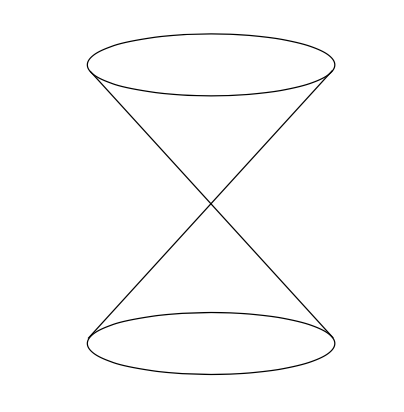
\includegraphics[scale=0.6]{quotientsubset}
    \end{center}
    
    \item Similarly, one can think of $\spc \C[x,y]_{(x,y)}$ as the shred of the affine plane near the origin.
    \begin{center}
    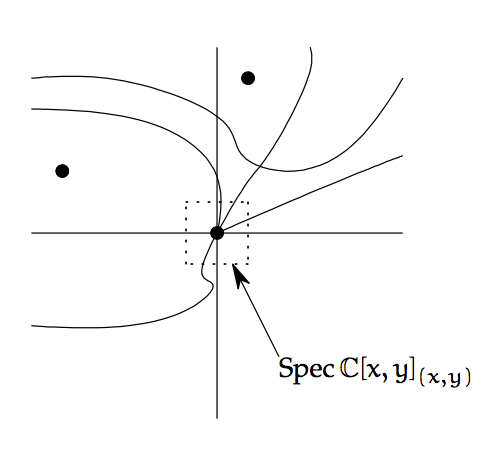
\includegraphics[scale=0.6]{localshred}
    \end{center}
    
    \item The space $\spc \C[x,y]_{y-x^2}$ can be thought of the affine plane, minus those points on the parabola $y - x^2$.
\end{itemize}
For more information on these examples, as well as more examples, see \cite{vakil}.
\end{example}
\pagebreak

%----------------------------------------------------------------------------------------
%----------------------------------------------------------------------------------------

\subsection{The Topology}

\begin{definition}\
\begin{itemize}
	\item If $S \subseteq A$, the \emph{vanishing set} of $S$ is the set
	\[
		V(S) := \{[\mathfrak{p}] \in \spc A \mid S \subseteq \mathfrak{p}\}.
	\]
	It is the set of all prime ideals containing $S$, i.e. the set of all points of $\spc A$ on which all the elements of $S$ are $0$.

	\item The \emph{Zariski topology} on $\spc A$ is defined by declaring $V(S)$ to be closed for all $S \subseteq A$.
\end{itemize}
\end{definition}

In fact, it is enough to consider only the vanishing sets of ideals.\\

\begin{lemma}
If $(S)$ is the ideal generated by $S$, then $V(S) = V((S))$.
\end{lemma}
\medskip

We should verify that the Zariski topology is actually a topology on $\spc A$.\\

\begin{proposition}
The Zariski topology is indeed a topology on $\spc A$. In particular,
\begin{enumerate}
	\item $\emptyset$ and $\spc A$ are both open subsets of $\spc A$.
    \item If $I_i$ is a collection of ideals, then $$\bigcap_i V(I_i) = V\left(\sum_i I_i\right).$$ 
    \item If $I_1,\ldots,I_n$ are ideals, then $$V(I_1) \cup \cdots \cup V(I_n) = V(I_1\cdots I_n).$$
\end{enumerate}
\end{proposition}
\hfill

It will be useful to have a base of open sets for the Zariski topology.\\

\begin{definition}
If $f \in A$, the \emph{distinguished open set} of $f$ is the set
\[
	D(f) := \{[\mathfrak{p}] \in \spc A \mid f \not\in \mathfrak{p}\}.
\]
\end{definition}
\hfill

\begin{proposition}
The distinguished open sets form a base of the Zariski topology.
\end{proposition}
\hfill

The following lemma states that the $\spc$ functor is in fact a contravariant functor from $\mathbf{Rng}$ to $\mathbf{Top}$.\\

\begin{lemma} \label{spctop}
If $B \to A$ is a map of rings, then the induced map of spectra $\spc A \to \spc B$ of Lemma \ref{spcset} is continuous.
\end{lemma}

%----------------------------------------------------------------------------------------
%----------------------------------------------------------------------------------------

\subsection{The Structure Sheaf}
To finish putting a geometric structure on a ring, we now define the structure sheaf. It suffices to define this sheaf on the base of distinguished sets, as it can then be extended to the entire space via Theorem \ref{basesheaf}.\\

\begin{definition}
Define $\mathcal{O}_{\spc A}(D(f))$ to be the localization of $A$ at the multiplicative set of functions that do not vanish outside of $V(f)$.
\end{definition}
\hfill

The following proposition offers a perhaps easier way to view $\mathcal{O}_{\spc A}(D(f))$.\\

\begin{proposition}
There is a natural isomorphism $A_f \simeq \mathcal{O}_{\spc A}(D(f))$.
\end{proposition}
\hfill

The next lemma is important in showing that $\mathcal{O}_{\spc A}(D(f))$ is a good definition.\\

\begin{lemma}
The ring $\mathcal{O}_{\spc A}(D(f))$ depends only on $D(f)$, not on $f$ itself.
\end{lemma}
\hfill

We now define the restriction maps.\\

\begin{definition}
If $D(f') \subseteq D(f)$, define
\[
	\operatorname{res}_{D(f),D(f')} : \mathcal{O}_{\spc A}(D(f)) \to \mathcal{O}_{\spc A}(D(f'))
\]
to be the natural map $A_f \to A_{f'}$.
\end{definition}
\hfill

\begin{theorem}
The above data gives a sheaf (of rings) on the distinguished base of $\spc A$, and hence a sheaf (of rings) on $\spc A$.
\end{theorem}
\hfill

At last comes our desired definition.\\

\begin{definition}
An \emph{affine scheme} is a ringed space $(\spc A, \mathcal{O}_{\spc A})$, where $\spc A$ is the spectrum of a ring $A$ endowed with the Zariski topology, and $\mathcal{O}_{\spc A}$ is the structure sheaf defined above.
\end{definition}

\begin{example}\
\begin{itemize}
	\item $\spc k$, where $k$ is a field, is just a single point.
    
    \item The points of $\spc \Z$ correspond to the prime numbers, along with an additional ``generic point'' $[(0)]$. (This generic point is present in every scheme, and has the strange property that it somehow lies near every other point, since the prime ideal $(0)$ is contained in every other prime ideal. This is one of the first indications that the Zariski topology is unusual.) One function on $\spc \Z$ is the number $100$, whose value at $[(3)]$ is $1$, and who has a double zero at $[(2)]$. (Indeed, any integer is a function on $\spc \Z$, and its value at a point is just its value mod that prime.) Another function on $\spc \Z$ is the rational function $27/4$, which has a double pole at $[(2)]$ and a triple zero at $[(3)]$, and whose value at $[(5)]$ is $27\times4^{-1} \equiv 2 \times (-1) \equiv 3$.
    \begin{center}
    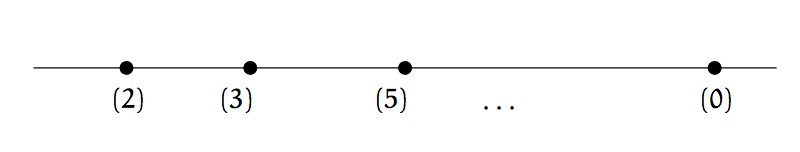
\includegraphics[scale=0.7]{specz}
    \end{center}
   
   \item The points of $\spc \R[x]$ correspond to prime ideals of the form $(0)$, $(x - a)$, and $(x^2 + ax + b)$, where $x^2 + ax + b \in \R[x]$ is irreducible. The space should be thought of as the complex plane, folded along the real axis, with Galois conjugate points glued together. The value of the function $f(x) = x^3 - 1$ at $[(x - 2)]$ is $7$, and the value of $f(x)$ at $x^2 + 1$ is $-x - 1$, which may be interpreted as $-i - 1$.
\end{itemize}
For more information on these examples, as well as more examples, see \cite{vakil}.
\end{example}

%----------------------------------------------------------------------------------------
%----------------------------------------------------------------------------------------

\subsection{The Category of Affine Schemes} \label{affschcat}
Observe that an affine scheme is a ringed space. A morphism of affine schemes is therefore a morphism of ringed spaces: a continuous map $\spc A \to \spc B$ together with a map $\mathcal{O}_{\spc B} \to \pi_*\mathcal{O}_{\spc A}$.\\

Note that one can easily recover a ring morphism from a morphism of affine schemes via the map
\[
B \simeq \Gamma(\mathcal{O}_{\spc B},\spc B) \longrightarrow \Gamma(\pi_*\mathcal{O}_{\spc A},\spc A) \simeq A.
\]

We would like to be able to move in the opposite direction: given a ring morphism $\pi^{\#} : B \to A$, how can we recover a morphism of affine schemes $\pi : (\spc A, \mathcal{O}_{\spc A}) \longrightarrow (\spc B, \mathcal{O}_{\spc B})$?\\

By Lemmas \ref{spcset} and \ref{spctop},  a ring morphism $\pi^{\#} : B \to A$ induces a map of spectra $\pi : \spc A \to \spc B$ given by $\pi([\mathfrak{p}]) = [(\pi^{\#})^{-1}(\mathfrak{p})]$. The next lemma gives the final component, a map of sheaves $\mathcal{O}_{\spc B} \longrightarrow \pi_*\mathcal{O}_{\spc A}$.\\ 

\begin{lemma} \label{spcsheaf}
If $\pi^{\#} : B \to A$ is a ring morphism and $D(g) \subseteq \spc B$ is a distinguished open set, define a map
\[
\mathcal{O}_{\spc B}(D(g)) \longrightarrow \mathcal{O}_{\spc A}(\pi^{-1}D(g)) = \mathcal{O}_{\spc A}(D(\pi^{\#}g)
\]
by the natural map $B_g \to A_{\pi^{\#}g}$ (induced by the universal property of localization). This map gives a well-defined (independent of representative $g$ of $D(g)$) morphism of sheaves on the distinguished base, and therefore a morphism of sheaves $\mathcal{O}_{\spc B} \to \pi_*\mathcal{O}_{\spc A}$.
\end{lemma}
\medskip

Having defined morphisms of affine schemes, we now have a category of affine schemes, which we shall denote $\mathbf{AffSch}$. It is a subcategory of the category of ringed spaces. Additionally, the $\spc$ functor may now be viewed as a functor from $\mathbf{Rng}$ to $\mathbf{AffSch}$. Note that we also have a functor $\Gamma$ from $\mathbf{AffSch}$ to $\mathbf{Rng}$; it sends an affine scheme $(\spc A,\mathcal{O}_{\spc A})$ to its ring of global sections $\Gamma(\mathcal{O}_{\spc A}, \spc A)$. 

\begin{remark}
More generally, $\spc$ is a functor from $\mathbf{Rng}$ to ringed spaces, and $\Gamma$ is a functor from ringed spaces to $\mathbf{Rng}$.
\end{remark}

\begin{lemma}
$\spc$ and $\Gamma$ are adjoint functors.
\end{lemma}
\medskip

The following theorem will anger the reader until the next section.\\

\begin{theorem}
The category $\mathbf{AffSch}$ of affine schemes is anti-equivalent to the category $\mathbf{Rng}$ of rings.
\end{theorem}

%----------------------------------------------------------------------------------------
%----------------------------------------------------------------------------------------
%----------------------------------------------------------------------------------------

\section{Schemes}
The point of the previous section, it turns out, was not to needlessly abstract rings to a mostly useless and complicated geometric structure, but rather to generalize them to a broader class of geometric structure known as a scheme. The definition of a scheme comes from gluing affine schemes together.\\

\begin{definition}
A \emph{scheme} is a ringed space $(X, \mathcal{O}_X)$ such that any point of $X$ has an open neighborhood $U$ such that $(U, \mathcal{O}_X\restriction_U)$ is an affine scheme.
\end{definition}

\begin{example}\
\begin{itemize}
	\item Any affine scheme is evidently a scheme.
    \item For a field $k$, let $A = k[x,y]$, and let $\mathbf{A}^2 = \spc A$, the \emph{affine plane over $k$}. Then $U = D(x) \cup D(y) = \mathbf{A}^2 - \{[(x,y)]\}$ is a distinguished open set, the \emph{affine plane minus the origin}. The space of functions on $U$ is the set of functions on $D(x)$ and $D(y)$ that agree on $D(x) \cap D(y) = D(xy)$. This is equivalent to considering $A_x \cap A_y$ in $A_{xy} = k(x,y)$. But the only rational functions who have both only powers of $x$ and only powers of $y$ in their denominators are the polynomials, so $A_x \cap A_y = A$, and therefore $\Gamma(U, \mathbf{A}^2) = k[x,y]$. Counterintuitively, although $\mathbf{A}^2$ is an affine scheme, $(U, \mathcal{O}_{\mathbf{A}^2}\restriction_U)$ is not, since the prime ideal $(x,y)$ does not cut out a point of $U$.
\end{itemize}
\end{example}

The next lemma is in fact quite important; it will be employed in the very definition of a morphism of schemes.\\

\begin{lemma}
A scheme is a locally ringed space.
\end{lemma}
\medskip

Of course, we can have subsets of schemes that are also schemes but are not affine schemes.\\

\begin{lemma}
If $(X, \mathcal{O}_X)$ is a scheme and $U$ is any open subset of $X$, then $(U, \mathcal{O}_X\restriction_U)$ is also a scheme.
\end{lemma}
\medskip

\begin{definition}
In the notation of the above lemma, $(U, \mathcal{O}_X\restriction_U)$ is called an \emph{open subscheme} of $X$. If $U$ is also an affine scheme, then we call $U$ an \emph{affine open subscheme}, or \emph{affine open subset}, or just \emph{affine open}.
\end{definition}

\begin{example}
If $A$ is a ring and $f \in A$, then $D(f)$ is an affine open subset of $\spc A$.
\end{example}

Although schemes are locally affine schemes, our definition does not describe how one can actually glue affine schemes together to get a scheme. The following proposition explains not only when one can glue affine schemes, but when one can glue schemes in general.\\

\begin{proposition}
Let $\{X_i\}_{i \in I}$ be a collection of schemes. Suppose $X_{ij} \subseteq X_i$ with $X_{ii} = X_i$ are open subschemes, and that there are isomorphisms $f_{ij} : X_{ij} \to X_{ji}$, for all $i,j \in I$. If the isomorphisms satisfy the \emph{cocycle condition} $f_{ik}\restriction_{X_{ij} \cap X_{ik}} = f_{jk}\restriction_{X_{ji} \cap X_{jk}} \circ f_{ij}\restriction_{X_{ij} \cap X_{ik}}$, then there is a unique scheme $X$ with open subsets isomorphic to each $X_i$ respecting the gluing data described.
\end{proposition}

\begin{example}\
\begin{itemize}
	\item For a field $k$, let $X = \spc k[t]$ and $Y = \spc k[u]$. Let $U = D(t) = \spc k[t,1/t]$ and $V = D(u) = \spc k[u,1/u]$. Gluing $X$ and $Y$ together along the isomorphism $U \simeq V$ given by $t \leftrightarrow u$ results in the \emph{affine line with doubled origin.} This is a scheme which is not affine.\\
    \begin{center}
    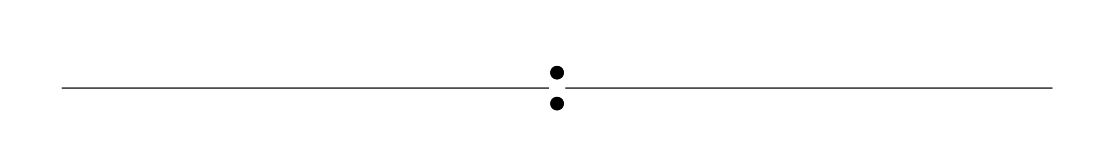
\includegraphics[scale=0.5]{afflinedouble}
    \end{center}
    
    \item Continuing with the same notation as the previous example, now glue $X$ and $Y$ together along the isomorphism $U \simeq V$ given by $t \leftrightarrow 1/u$. This results in what is known as the \emph{projective line over $k$}, and is also not affine. This is the first example of a projective scheme. Projective schemes are vastly important and perhaps among the most commonly studied types of schemes. We will not use them much in this paper, and refer the reader to \cite{vakil} for more information.\\
    \begin{center}
    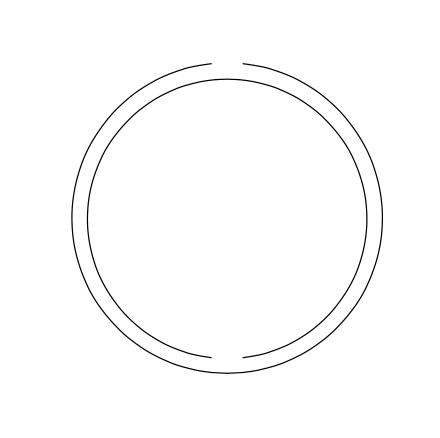
\includegraphics[scale=0.5]{projline}
    \end{center}
\end{itemize}
\end{example}

%----------------------------------------------------------------------------------------
%----------------------------------------------------------------------------------------
%----------------------------------------------------------------------------------------

\section{Morphisms of Schemes} \label{schememor}
Since a scheme is a ringed space that locally looks like an affine scheme, we should hope that a morphism of schemes is a morphism of ringed spaces that locally looks like a morphism of affine schemes. More precisely, if $\pi : X \to Y$ is a morphism of schemes, and $\spc A \subseteq X$ and $\spc B \subseteq Y$, with $\pi(\spc A) \subseteq \spc B$, then the induced map $\spc A \to \spc B$ should be a morphism of affine schemes as described in Section \ref{affschcat}.\\


There should also be some inherent geometry in morphisms of schemes. This geometry is motivated by the theory of differentiable manifolds, where one can pull back a differentiable function to another differentiable function. Translating this notion to the language of schemes requires one to hardwire this information into a pullback map $\mathcal{O}_Y \to \pi_*\mathcal{O}_X$, leading to a morphism of ringed spaces. Unfortunately, this is not sufficient to define morphisms of schemes, as it is possible to have morphisms of ringed spaces $\spc B \to \spc A$ which do not arise from morphisms of rings $A \to B$---breaking our algebraic motivation. (See \cite{vakil} for more information on this and the geometric motivation.) To fix this issue, we require morphisms of schemes to be morphisms of locally ringed spaces.\\

\begin{definition}
If $X$ and $Y$ are schemes, then a \emph{morphism of schemes} is a morphism $\pi : X \to Y$ as locally ringed spaces.\\

The category of schemes is denoted $\mathbf{Sch}$.
\end{definition}

Note that $\mathbf{AffSch}$ is a full subcategory of of $\mathbf{Sch}$.\\

The following proposition is unsurprising, since the category of affine schemes is dual to the category of rings, and morphisms of affine schemes can be glued to create morphisms of schemes, by Lemma \ref{gluersmor}.\\

\begin{proposition} \label{finsch}
The affine scheme $\spc \Z$ is final in $\mathbf{Sch}$.
\end{proposition}

%----------------------------------------------------------------------------------------
%----------------------------------------------------------------------------------------

\subsection{Morphisms Over a Scheme and Related Concepts}

\subsubsection{Base Schemes}
As if the category of schemes was not complicated enough, we now define the category of schemes over a base scheme.\\

\begin{definition}
Fix a scheme $X$, and let $\mathbf{Sch}_X$ be the category defined as follows. The objects are morphisms of schemes $Y \to X$, and the morphisms are commutative diagrams of the following form.
\[
\begin{tikzcd}
Y \ar[rr] \ar[rd] & & Z \ar[ld] \\
& X
\end{tikzcd}
\]
An object in the category $\mathbf{Sch}_X$ is often referred to as an \emph{$X$-scheme}, and $X$ is called a \emph{base scheme}.\\

If $X = \spc A$ for some ring $A$, we will lazily refer to $\mathbf{Sch}_X$ as $\mathbf{Sch}_A$, and write $A$-scheme for $\spc A$-scheme.
\end{definition}

Note that by Proposition \ref{finsch}, the category of schemes is isomorphic to the category of $\Z$-schemes.

\subsubsection{Scheme-Valued Points}
We now discuss scheme-valued points; this is an extremely important concept.\\

\begin{definition}
Let $Z$ be a scheme. The \emph{$Z$-valued points} of a scheme $X$, denoted $X(Z)$, are defined to be the morphisms $Z \to X$.\\

If $A$ is a ring, the \emph{$A$-valued points} of a scheme $X$, denoted $X(A)$ are the $\spc A$-valued points of $X$. Of particular interest is the case where $A$ is a field; when $A = \overline{k}$ is an algebraically closed field, the $\overline{k}$-valued points of a scheme $X$ are called \emph{geometric points} of $X$.
\end{definition}

Note that if one is working over a base scheme $Y$, then in the above definition there is an implicit structure map $Z \to B$, so $Z$-valued points of $X$ look like commutative diagrams
\[
\begin{tikzcd}
Z \ar[rd] \ar[rr] & & X \ar[ld] \\ & Y.
\end{tikzcd}
\]

The following lemma gives one reason why scheme-valued points are useful.\\

\begin{lemma}
The $A$-valued points of an affine scheme $\spc \Z[x_1,\ldots,x_n]/(f_1,\ldots,f_r)$ are precisely the solutions to the equations
\[
f_1(x_1,\ldots,x_n) = \cdots = f_r(x_1,\ldots,x_n) = 0
\]
in $A$.
\end{lemma}
\medskip

\begin{example}
The rational points on the elliptic curve $y^2 = x^3 + x$ are precisely the $\Q$-valued points of $\spc \Z[x,y]/(y^2 - x^3 - x)$. The integral solutions are the $\Z$-valued points.
\end{example}

\begin{remark}
An important concept is the \emph{functor of points} $h_X$, mapping each scheme $Z$ to the set $X(Z)$. This gives an alternative way to think about schemes and the definition of schemes. We will not use it in any essential way.
\end{remark}

\subsubsection{Fibres and Fibred Products}

The reader should hopefully require little convincing of the importance of fibred products. Fibred products will play an essential role in our later discussion of Galois theory for schemes, where we use them to construct the ``fibre functor''.\\

For a scheme $Z$, the product of two objects in $\mathbf{Sch}_Z$ is the fibred product of two schemes over $Z$. In particular for a scheme $W$, the $W$-valued points behave nicely under fibred products, since by definition (and Yoneda's Lemma)

\[
\operatorname{Hom}(W,X \times_Z Y) = \operatorname{Hom}(W,X) \times_{\operatorname{Hom}(W,Z)} \operatorname{Hom}(W, Y),
\]
and $W$-valued points of $X$ are just elements of $\operatorname{Hom}(W,X)$.\\

Fibred products in the affine case are unsurprising. Recall that $A \otimes_C B$ is the fibred coproduct in the category of rings, and $\spc$ is a contravariant functor from $\mathbf{Rng}$ to $\mathbf{AffSch}$ (in fact, an anti-equivalence.) The following lemma hence follows easily.\\

\begin{lemma}
If $C \to A$ and $C \to B$ are ring maps, then
\[
\spc A \times_{\spc C} \spc B \simeq \spc (A \otimes_C B).
\]
\end{lemma}
\medskip

To construct fibred products for general schemes, one cuts everything into affine subsets, takes the fibred product there, then glues everything back together.\\

\begin{theorem} \label{fibexist}
Suppose $\alpha : X \to Z$ and $\beta : Y \to Z$ are morphisms of schemes. Then the fibred product
\[
\begin{tikzcd}
X \times_Z Y \ar[d, "\beta'", swap] \ar[r, "\alpha'"] & Y \ar[d, "\beta"] \\
X \ar[r, "\alpha"] & Z
\end{tikzcd}
\]
exists in the category of schemes.
\end{theorem}
\medskip

Fibred products offer a way to change to a different base scheme. In fact, they give a functor $\mathbf{Sch}_Z \to \mathbf{Sch}_X$.\\

\begin{definition}
In the language of Theorem \ref{fibexist}, we say that $\beta'$ is the \emph{base change} of $\beta$ via $\alpha$, and similarly for $\alpha'$.
\end{definition}


Of particular interest to us will be the special case of the fibre of a morphism. Recall that for a map of topological spaces $f: Y \to Z$, the fibre of a point $p \in Z$ is the set-theoretic fibre $f^{-1}(p)$, with the induced topology. Equivalently, the fibre of $p$ is the fibred product $\{p\} \times_Z Y$. More generally, for $\pi : X \to Z$, the fibre of the map $X \times_Z Y \to X$ over a point $p$ in $X$ is naturally identified as the fibre of $Y \to Z$ over $\pi(p)$. Using this motivation from topology, we have the following natural definition of fibres for schemes.\\

\begin{definition}
Let $p$ be a point of a scheme $Z$, with residue field $k$, and consider the map $\spc k \to Z$ sending $\spc k$ to $p$, with the natural isomorphism of residue fields. If $g : Y \to Z$ is any morphism of schemes, then the base change of $g$ with the map $\spc k \to Z$ is the \emph{fibre of $g$ above/over $p$}. The fibre is sometimes denoted $g^{-1}(p)$ or $Y_p$.\\

If $z : \spc \overline{k} \to Z$ is a geometric point of $Z$, then the fibre of a morphism $g : Y \to Z$ over $z$ is referred to as a \emph{geometric fibre}.
\end{definition}
%----------------------------------------------------------------------------------------
%----------------------------------------------------------------------------------------

\subsection{Important Classes of Morphisms}
We now give several examples of useful classes of morphisms. The hope is that all reasonable classes of morphisms share the following properties.
\begin{enumerate}[label=(\roman*)]
	\item They are \emph{local on the target}: if $\pi : X \to Y$ is in the class, then for any open subset $V \subseteq Y$, the restricted morphism $\pi^{-1}(V) \to V$ is in the class; and if $\pi : X \to Y$ is a morphism and $\{V_i\}$ is an open cover of $Y$ such that the restrictions $\pi^{-1}(V_i) \to V_i$ are all in the class, then $\pi$ is in the class.
    \item They are closed under ``base change'' (or ``pullback,'' or ``fibred product'').
    \item They are closed under composition: if $\pi : X \to Y$ and $\rho : Y \to Z$ are in the class, then $\rho \circ \pi$ is in the class.
\end{enumerate}

%----------------------------------------------------------------------------------------

\subsubsection{Some Straightforward Types of Morphisms}
\begin{definition}
A morphism $\pi : X \to Y$ is \emph{quasicompact} if for every affine open subset $\spc B \subseteq Y$, the preimage $\pi^{-1}(\spc B)$ is a quasicompact scheme.
\end{definition}

\begin{definition}
A morphism $\pi : X \to Y$ is \emph{quasiseparated} if for every affine open subset $\spc B \subseteq Y$, the preimage $\pi^{-1}(\spc B)$ is a quasiseparated scheme (meaning the intersection of any two quasicompact open sets is quasicompact).
\end{definition}

\begin{definition}
A morphism $\pi : X \to Y$ is \emph{affine} if for every affine open subset $\spc B \subseteq Y$, the preimage $\pi^{-1}(\spc B)$ is an affine open subset of $X$.
\end{definition}

\begin{definition}
A morphism $\pi : X \to Y$ is \emph{finite} if for every affine open subset $\spc B \subseteq Y$, the preimage $\pi^{-1}(\spc B)$ is the spectrum of a finite $B$-algebra.
\end{definition}

Note that finite morphisms are affine.

\begin{definition}
A morphism $\pi : X \to Y$ is \emph{locally of finite type} if for every affine open subset $\spc B \subseteq Y$ and every affine open subset $\spc A \subseteq \pi^{-1}(\spc B)$, the induced morphism $B \to A$ of rings expresses $A$ as a finitely generated $B$-algebra.
\end{definition}

\begin{definition}
A morphism $\pi : X \to Y$ is \emph{of finite type} if it is locally of finite type and quasicompact.
\end{definition}

\begin{proposition}
A morphism is finite if and only if it is integral and of finite type.
\end{proposition}

\begin{proposition}
All of the types of morphisms defined above satisfy desired properties (i)--(iii).
\end{proposition}

%----------------------------------------------------------------------------------------

\subsubsection{Open and Closed Embeddings}

Although a scheme has a topology, it is often not particularly useful to speak of the open and closed subsets of this topology directly. Open and closed embeddings are meant to be the scheme theoretic analogues of open and closed subsets, respectively.\\

\begin{definition}
A morphism $\pi : (X, \mathcal{O}_X) \to (Y, \mathcal{O}_Y)$ is an \emph{open embedding}, or \emph{open immersion}, if it factors as
\[
\begin{tikzcd}
(X, \mathcal{O}_X) \ar[r, "\rho", "\sim"'] & (U,\mathcal{O}_Y\restriction_U) \ar[r, hook, "\tau"] & (Y, \mathcal{O}_Y),
\end{tikzcd}
\]
where $\rho$ is an isomorphism and $\tau : U \hookrightarrow Y$ is the inclusion of an open set.
\end{definition}

\begin{proposition}
Open embeddings satisfy properties (i)-(iii) of scheme morphisms.
\end{proposition}

\begin{definition}
A morphism $\pi : X \to Y$ is a \emph{closed embedding}, or \emph{closed immersion}, if $\pi$ is affine, and for each affine open subset $\spc B \subseteq Y$ with $\pi^{-1}(\spc B) \simeq \spc A$, the map $B \to A$ is surjective.
\end{definition}

\begin{proposition}
Closed embeddings are finite and satisfy properties (i)-(iii) of scheme morphisms.
\end{proposition}
%----------------------------------------------------------------------------------------

\subsubsection{(Finite) \'Etale}

Recall that an \'etale map of topological spaces is a local homeomorphism, i.e., $f : X \to Y$ is \'etale if each $p \in X$ has an open neighborhood $U \ni p$ such that $f(U)$ is open and $f\restriction_U : U \to f(U)$ is a homeomorphism. An \'etale map of schemes is an attempt to translate this notion to the language of schemes. Given the algebraic nature of schemes, this translation will naturally require an algebraic condition in addition to the geometric one. The definition of an \'etale map itself is complicated\footnote{Plus, a finite \'etale morphism is, according to some definitions, not just an \'etale morphism that is finite, but rather an \'etale morphism that is finitely presented. What jerk comes up with this stuff?} and we will not use it in any essential way; therefore we restrict our attention to finite \'etale maps. A finite \'etale cover is the correct analogue in scheme theory of a finite cover in topology.\\

Fix a field $k$ with algebraic closure $\overline{k}$. Recall (Proposition \ref{etalealgebra}) that a $k$-algebra $A$ is finite \'etale if and only if $A \otimes_{k} \overline{k} \simeq \overline{k}^n$ for some $n \in \Z^+$. Translating to the language of schemes, we have
\[
	\spc (A \otimes_k \overline{k}) \simeq \spc (\overline{k}^n) \simeq \coprod_{i=1}^{n} \spc \overline{k}.
\]
This suggests the following definition for a finite \'etale morphism.\\

\begin{definition}
Let $\phi : Y \to X$ be a morphism of schemes. If the geometric fibres of $\phi$ are of the form $\coprod_{i=1}^{n} \spc \overline{k}$ for some algebraically closed field $\overline{k}$, then we say that $\phi$ is \emph{finite \'etale}.\\

If $\phi$ is additionally surjective, we say that $\phi$ is a \emph{finite \'etale cover}.
\end{definition}

In the above definition, we see how finite \'etale cover of schemes are a translation of finite covers of topological spaces, with an additional algebraic condition. There are several other equivalent definitions of finite \'etale covers, as seen in the following proposition.\\

\begin{proposition}
Let $\phi : Y \to X$ be a morphism of schemes. Then the following are equivalent:
\begin{enumerate}
	\item $\phi$ is finite \'etale.
    \item There is a covering of $Y$ by open affine subsets $\spc A_i$, such that $\pi^{-1}(\spc A_i)$ is of the form $\spc B_i$, where $B_i$ is an \'etale $A_i$-algebra.
\end{enumerate}
\end{proposition}

\begin{example}\
\begin{itemize}
	\item If $X$ is a scheme, then the disjoint union $X \coprod X \coprod \cdots \coprod X$ of $n$ copies of $X$, with the natural morphism to $X$, is a finite \'etale covering of $X$. This follows because the preimage of an affine subscheme $\spc A$ is just $\coprod_{i=1}^{n} \spc A = \spc A^n$, and $A^n$ is clearly a finite \'etale $A$-algebra.\\

	If $X = \spc \Z$, all finite \'etale covers are of this form, which will be proven in \ref{etalefun}.

	\item If $K$ is a field, then the finite \'etale coverings of $\spc K$ are the maps $\coprod_{i=1}^{n} \spc B_i \to K$, where $B_i$ is a finite separable field extension of $K$.
    
    \item Any open embedding is finite \'etale.
\end{itemize}
\end{example}

Just as finite covers of topological spaces are locally trivial, finite \'etale covers of schemes are also locally trivial. Call a finite \'etale cover $\phi : Y \to X$ \emph{trivial} if $Y$ as a scheme over $X$ is isomorphic to a finite disjoint union of copies of $X$, and the map $\phi$ restricts to the identity on each component.\\

\begin{lemma}
Let $X$ be a connected scheme and $\phi : Y \to X$ be an affine surjective morphism. Then $\phi$ is a finite \'etale cover if and only if there is a finite, locally free, and surjective $\psi : Z \to X$ such that $Y \times_X Z$ is a trivial cover of $Y$.
\end{lemma}
\hfill

We now record some useful properties of finite \'etale morphisms that will come into play in Chapter \ref{galois}.\\

\begin{lemma}\ \label{etalefibre}
\begin{enumerate}[label=$\blacktriangleright$]
	\item If $Y \to X$ and $Z \to Y$ are finite \'etale, then the composed morphism $Z \to Y \to X$ is finite \'etale.
    \item Let $f : Y \to X$ and $g : Z \to X$ be finite \'etale morphisms, and $h : Y \to Z$ a morphism with $f = gh$. Then $h$ is finite \'etale.
	\item Suppose $Y \to X$ is a finite \'etale morphism and $W \to X$ is any morphism of schemes. Then the morphism $Y \times_X W \to W$ is finite \'etale.
\end{enumerate}
\end{lemma}

%----------------------------------------------------------------------------------------
%----------------------------------------------------------------------------------------
%----------------------------------------------------------------------------------------
%	CHAPTER - Galois Theory
%----------------------------------------------------------------------------------------
%----------------------------------------------------------------------------------------
%----------------------------------------------------------------------------------------

\chapter{Galois Theory} \label{galois}

The classical theorem of Galois Theory gives a beautiful correspondence between fields and groups. Analogous theorems have since been developed for wider classes of objects. In this chapter we study such correspondences, and the connection between them, from a geometric viewpoint. \\

In the first section, we describe Galois theory for fields, starting with finite field extensions and then moving on to infinite Galois theory and Grothendieck's formulation in terms of \'etale algebras.
In the second section, we describe the classification of covering spaces of a topological space, offering two theorems giving a Galois correspondence for certain spaces and certain types of coverings.
The third section focuses on Galois theory for schemes, developing it from the motivation of the first two sections. We end the chapter with a section on Galois categories and fibre functors, which offer a powerful generalization from which the theorems of the first three sections are easily deduced.

%----------------------------------------------------------------------------------------
%----------------------------------------------------------------------------------------
%----------------------------------------------------------------------------------------

\section{Fields} \label{secgalfld}

The classical theorem of Galois theory for finite extensions is usually phrased as follows.\\

\begin{theorem}[Fundamental Theorem of Galois Theory---Finite Version] \label{galfinfld}
Let $k \subseteq L$ be a finite Galois extension. The maps
\[
F \mapsto \operatorname{Aut}_F(L) \;\; \text{ and } \;\; H \mapsto L^H
\]
yield an inclusion reversing bijection
\[
\left\lbrace \text{intermediate extensions } k \subseteq F \subseteq L \right\rbrace \longleftrightarrow \left\lbrace \text{subgroups } H \leq \operatorname{Gal}_k(L) \right\rbrace.
\]
Let $k \subseteq F \subseteq L$ be an intermediate extension, and let $H$ be the group corresponding to $F$ under the described bijection. Then
\begin{enumerate}
	\item The extension $F \subseteq L$ is always Galois.
    \item We have $[F : k] = [\operatorname{Gal}_k(L) : H]$.
    \item The extension $k \subseteq F$ is Galois if and only if $H \trianglelefteq \operatorname{Gal}_k(F)$, and if so then $\operatorname{Gal}_k(F) \simeq \operatorname{Gal}_k(F)/H$.
\end{enumerate}
\end{theorem}

\begin{remark}
The modern viewpoint would have us viewing the above theorem as an equivalence of categories between the category of isomorphism classes of intermediate extensions of $k \to L$ , partially ordered by inclusion, and the opposite category of subgroups of $\operatorname{Gal}_k(L)$.
\end{remark}

\begin{example}
Consider the field extension $\Q \subseteq \Q(\sqrt[3]{2},\zeta_3)$, where $\zeta_3$ is a primitive third root of unity. This is a splitting field extension for $x^3 - 2$ and is hence Galois. The Galois group $G = \operatorname{Gal}_{\Q}(\Q(\sqrt[3]{2},\zeta_3)$ is generated by the automorphisms $\sigma$ $\tau$, where $\sigma$ is defined by $\sqrt[3]{2} \mapsto \zeta_3\sqrt[3]{2}$ and $\zeta_3 \mapsto \zeta_3$, and $\tau$ is defined by $\sqrt[3]{2} \mapsto \sqrt[3]{2}$ and $\zeta_3 \mapsto \zeta_3^2$, which yields that the Galois group $G$ is isomorphic to $S_3$. We have the following lattices of intermediate field extensions and corresponding subgroups.
\pagebreak

\begin{center} \textbf{Fields} \end{center}
\[
\begin{tikzcd}
& & \Q(\sqrt[3]{2}, \zeta_3) & \\
\Q(\zeta_3) \ar[urr, "\text{Galois}"] & \Q(\sqrt[3]{2}) \ar[ur, "\text{Galois}", swap] & \Q(\zeta_3^2\sqrt[3]{2}) \ar[u, "\text{Galois}", swap] & \Q(\zeta_3\sqrt[3]{2}) \ar[ul, "\text{Galois}", swap] \\
& & \Q \ar[ull, "\text{Galois}"] \ar[ul] \ar[u] \ar[ur] &
\end{tikzcd}
\]
\begin{center} \textbf{Groups} \end{center}
\[
\begin{tikzcd}
& & \{1\} \ar[lld] \ar[ld] \ar[d] \ar[rd] & \\
\{1,\sigma,\sigma^2\} \ar[rrd] & \{1,\tau\} \ar[rd] & \{1, \sigma\tau\} \ar[d] & \{1,\sigma^2\tau\} \ar[ld] \\
& & \{1,\sigma,\sigma^2,\tau,\sigma \tau, \sigma^2\tau\} &
\end{tikzcd}
\]
\end{example}

Our first task is to generalize Theorem \ref{galfinfld} to infinite Galois extensions. Such work was initially done by Wolfgang Krull.\\

\begin{lemma}
Let $k \to L$ be a (possibly infinite) Galois extension. Denote by $\mathcal{I}$ the category of finite intermediate Galois extensions $k \to F \to L$, partially ordered by inclusion. Then $\operatorname{Gal}_k(L) \simeq \varprojlim_{F \in \mathcal{I}} \operatorname{Gal}_k(F)$. In particular, since $\operatorname{Gal}_k(F)$ is finite for each $F \in \mathcal{I}$, the Galois group $\operatorname{Gal}_k(L)$ is a profinite group.
\end{lemma}
\hfill

As a consequence of the above lemma, along with Theorem \ref{profin}, the group $\operatorname{Gal}_k(F)$ has a topology under which it is compact and totally disconnected. This topology is called the \emph{Krull topology}, after Wolfgang Krull.\\

\begin{theorem}[Fundamental Theorem of Galois Theory---Infinite Version] \label{galinffld}
Let $k \subseteq L$ be a (possibly infinite) Galois extension. The maps
\[
F \mapsto \operatorname{Aut}_F(L) \;\; \text{ and } H \mapsto L^H
\]
yield an inclusion reversing bijection
\[
\left\lbrace \text{intermediate extensions } k \subseteq F \subseteq L \right\rbrace \longleftrightarrow \left\lbrace \text{closed subgroups } H \leq \operatorname{Gal}_k(L) \right\rbrace.
\]
Let $k \subseteq F \subseteq L$ be an intermediate extension, and let $H$ be the group corresponding to $F$ under the described bijection. Then
\begin{enumerate}
	\item The extension $F \subseteq L$ is always Galois.
	\item The extension $k \subseteq F$ is finite if and only if $H$ is open. If so, then $[F : k] = [\operatorname{Gal}_k(L) : H]$.
    \item The extension $k \subseteq F$ is Galois if and only if $H \trianglelefteq \operatorname{Gal}_k(F)$. If so, then $\operatorname{Gal}_k(F) \simeq \operatorname{Gal}_k(F)/H$ as topological groups.
\end{enumerate}
\end{theorem}

\begin{remark}
As in the finite case, the above theorem could have been phrased in categorical terms, with similar caveats.
\end{remark}

\begin{example}
Let $\mathbf{F}_q$ be a finite field of order $q$. The finite extensions of $\mathbf{F}_q$ in $\overline{\mathbf{F}_q}$ are the fields $\mathbf{F}_{q^n} = \{\alpha \in \mathbf{F}_q \mid \alpha^n = \alpha\}$ for each $n \in \Z^+$. The Galois group of each $\mathbf{F}_q^n$ is isomorphic to $\Z/n\Z$ with generator $\alpha \mapsto \alpha^q$, the Frobenius automorphism. By taking projective limits, we find that the absolute Galois group of $\mathbf{F}_q$ is isomorphic to $\hat{\Z}$. One can show that $\hat{\Z}$ contains $\Z$ as a dense, and hence not closed subgroup. This implies that Theorem \ref{galinffld} does indeed offer something different in the infinite case than in the finite case---there are subgroups of the absolute Galois group which are not included in the described bijection.
\end{example}

In our spirit of generalization, even infinite Galois theory is not enough. We now describe another generalization of Galois theory, first developed by Grothendieck.\\

\begin{theorem}[Grothendieck's Formulation of Galois Theory] \label{galfldgrt}
Let $k$ be a field with algebraic closure $\overline{k}$ and fixed separable closure $k_s \subseteq \overline{k}$, and let $\pi = \operatorname{Gal}_k(k_s)$ be its absolute Galois group. Then the category $_k\mathbf{Et}$ of \'etale $k$-algebras is anti-equivalent to the category $\xsets{\pi}$ of finite sets with a continuous action of $\pi$.
\end{theorem}

The anti-equivalence of Theorem \ref{galfldgrt} is given by the functors $_k\mathbf{Et} \to \xsets{\pi}$ sending each \'etale $k$-algebra $A$ to the finite set $\Mor_k(A,k_s)$, and $\xsets{\pi} \to _k\mathbf{Et}$ sending each $\pi$-set $E$ to the $k$-algebra $\Mor_{\pi}(E,k_s)$. Of course, it must be proved that $\Mor_k(A,k_s)$ is actually a $\pi$-set and that $\Mor_{\pi}(E,k_s)$ is actually an \'etale $k$-algebra.\\
 
Under the anti-equivalence of Theorem \ref{galfldgrt}, separable field extensions correspond to sets with transitive $\pi$-action, and Galois extensions correspond to $\pi$-sets isomorphic to finite quotients of $\pi$. In this way, we see how Theorem \ref{galfldgrt} is a generalization of Theorems \ref{galfinfld} and \ref{galinffld}.

%----------------------------------------------------------------------------------------
%----------------------------------------------------------------------------------------
%----------------------------------------------------------------------------------------

\section{Topological Spaces} \label{secgaltop}
Grothendieck's formulation of Galois theory may at first seem poorly motivated: what inspired him to generalize this theorem to some abstract nonsense with \'etale algebras? In fact, his viewpoint offers a natural connection to a broader class of Galois theories. Indeed, in Theorem \ref{galfldgrt}, we essentially view $k$ as a point, the base point, and each \'etale $k$-algebra as a finite discrete set of points mapping to this base point. (This is stronger than analogy: we will see this is \emph{precisely} what is happening, once we rephrase things in the language of schemes.) One natural generalization of this situation would be to consider not just a singular base point, but an entire topological space.\\

Just as it is too hopeful to ask to classify \emph{any} field extension, it is too hopeful to ask to classify all the coverings of \emph{any} topological space. The usual adjustment leads to the following theorem.\\

\begin{theorem} \label{galtop1}
Let $X$ be a connected, locally path connected, and semilocally simply connected topological space. Then the category of coverings of $X$ is equivalent to the category of $\pi_1(X)\operatorname{-sets}$, where $\pi_1(X)$ is the fundamental group of $X$.
\end{theorem}

Theorem \ref{galtop1} is often reformulated as an equivalence between the category of coverings of $X$ and the category of conjugacy classes of subgroups of $\pi_1(X)$. For a further discussion of Theorem \ref{galtop1}, see \cite{munkres} or \cite{massey}.\\

This theorem, however, is weaker in analogy with our other theorems than it could be. The fundamental group $\pi(X)$ of Theorem \ref{galtop1} has no topology, and the $\pi(X)\operatorname{-sets}$ need not be finite---two characteristics which always hold for our other theorems. Seeking a closer analogy leads us to develop the following theorem, which classifies finite coverings of a much larger class of topological spaces.\\

\begin{theorem} \label{galtop2}
Let $X$ be a connected topological space. Then there is a profinite group $\hat{\pi}(X)$, uniquely determined up to isomorphism, such that the category of finite coverings of $X$ is equivalent to the category $\xsets{\hat{\pi}(X)}$ of finite sets on which $\hat{\pi}(X)$ acts continuously.
\end{theorem}

We will later see that in the above theorem, the profinite group $\hat{\pi}(X)$ is computed as the automorphism group of a ``fibre functor,'' dependent on a choice of basepoint $x$. This plays an analogous role to the Galois group of the separable closure in Theorem \ref{galfldgrt}, the choice of separable closure playing the role of the choice of basepoint. In fact, this is stronger than analogy: we will see that both are specific instances of a more general construction.

%----------------------------------------------------------------------------------------
%----------------------------------------------------------------------------------------
%----------------------------------------------------------------------------------------

\section{Schemes} \label{secgalsch}
We come now to our penultimate generalization: schemes. In this section we will explain the fundamental theorem of Galois theory for schemes, and see how it relates to the theorems of field theory and topology.\\

As a first step, we translate Grothendieck's formulation of Galois theory, Theorem \ref{galfldgrt}, to the language of schemes. This is easy to do, as should be no surprise since schemes also come from Grothendieck.\\

As before, fix a field $k$ with algebraic closure $\overline{k}$ and separable closure $k_s \subseteq \overline{k}$. Consider the $\spc$ functor from $_k\mathbf{Et}$ to $\mathbf{Sch}_k$. It sends each \'etale $k$-algebra $A$ with morphism $k \to A$ to $\spc A$ with morphism $\spc A \to \spc k$; essentially by definition this morphism is finite \'etale. So in fact, we can speak of $\spc$ as a functor from $_k\mathbf{Et}$ to the subcategory $\mathbf{FEt}_k$ of $\mathbf{Sch}_k$. The global section functor $\Gamma$ evidently gives an adjoint functor to $\spc$, as in Section \ref{affschcat}, defining an anti-equivalence of categories between $_k\mathbf{Et}$ and $\mathbf{FEt}_k$. We can therefore rephrase Theorem \ref{galfldgrt} as follows.\\

\begin{theorem} \label{galaffsch}
Let $k$ be a field with algebraic closure $\overline{k}$ and fixed separable closure $k_s \subseteq \overline{k}$, and let $\pi = \operatorname{Gal}_k(k_s)$ be its absolute Galois group. Then the category $\mathbf{FEt}_k$ of finite \'etale coverings of $\spc k$ is equivalent to the category $\xsets{\pi}$ of finite sets with a continuous action of $\pi$.
\end{theorem}
\medskip

The above theorem gives validity to viewing the field $k$ as a single point ($\spc k$), and each \'etale $k$-algebra is a finite set of points ($\prod \spc B_i$) mapping to $\spc k$.\\

The next step in our generalization is to classify finite \'etale covers not just of $\spc k$, but of any connected scheme.\\

\begin{theorem}[Galois Theory for Schemes] \label{galsch}
Let $X$ be a connected scheme. Then there exists a profinite group $\pi = \pi(X)$, uniquely determined up to isomorphism, such that the category $\mathbf{FEt}_X$ of finite \'etale coverings of $X$ is equivalent to the category $\pi$-$\mathbf{sets}$ of finite sets on which $\pi$ acts continuously.
\end{theorem}

\begin{remark}
One potential approach to proving Theorem \ref{galsch} would be to somehow use Theorem \ref{galaffsch}, looking at geometric points of the scheme $X$ and gluing morphisms together. We have not investigated if this approach actually works. We will see, in Section \ref{galcat} a more abstract approach offering an elegant proof of Theorem \ref{galsch}.
\end{remark}

The profinite group $\pi$ in Theorem \ref{galsch} is known as the \emph{\'etale fundamental group}, or \emph{algebraic fundamental group}. Examples of Theorem \ref{galsch} will be given in the next section, following a discussion of Galois categories and the \'etale fundamental group.

\section{Galois Categories} \label{galcat}

In generalizing Galois theory to \'etale algebras, topological spaces, and then to schemes, we saw a common theme of defining a profinite group by mapping each cover to its fibre over a fixed basepoint. This suggests a natural definition of a category, along with a fibre functor, that together satisfy a certain set of axioms allowing a Galois correspondence to occur.\\

\begin{definition}
Let $\mathcal{C}$ be a category and $F : \mathcal{C} \to \mathbf{sets}$ be a functor. We say that $\mathcal{C}$ is a \emph{Galois category} with \emph{fibre functor} $F$ if the following six axioms are satisfied.
\begin{enumerate}
	\item There is a final object in $\mathcal{C}$, and the fibred product of any two objects over a third exists.
    \item There is an initial object in $\mathcal{C}$, finite coproducts exist, and for any object in $\mathcal{C}$, the quotient by a finite group of automorphisms exists.
    \item Any morphism $u$ in $\mathcal{C}$ can be written as $u = u'u''$ where $u''$ is an epimorphism and $u'$ is a monomorphism. Further, any monomorphism $X \to Y$ is an isomorphism of $X$ with a direct summand of $Y$.
    \item The functor $F$ maps final objects to final objects and commutes with fibred products.
    \item The functor $F$ commutes with finite coproducts and quotients, and maps epimorphisms to epimorphisms.
    \item If $u$ is a morphism in $\mathcal{C}$ such that $F(u)$ is an isomorphism, then $u$ is an isomorphism.
\end{enumerate}
\end{definition}

\begin{example}[Prototypical examples of a Galois category]\
\begin{itemize}
	\item The category $\mathbf{sets}$ is a Galois category with fibre functor $F = id_{\mathbf{sets}}$.
	\item Let $\pi$ be a profinite group. The category $\xsets{\pi}$ of finite sets with a continuous action of $\pi$ is a Galois category with fibre functor $F : \xsets{\pi} \to \mathbf{sets}$ the forgetful functor.
\end{itemize}
\end{example}

Fix an essentially small\footnote{An essenially small category is category which is equivalent to one whose objects form a set. The hypothesis that $\mathcal{C}$ is essentially small is necessary to form an equivalence between $\mathcal{C}$ and an essentially small category $\xsets{\pi}$.} Galois category $\mathcal{C}$ with fibre functor $F$. For each $X \in \mathcal{C}$, let $S_{F(X)}$ denote the group of permutations of $F(X)$. Note that $F(X)$ lies in $\mathbf{sets}$ and is therefore finite, so $S_{F(X)}$ is also finite. We can thus consider the automorphism group of the functor $F$ as a subgroup $\Aut(F) \leq \prod_X S_{F(X)}$.\\

Endow each $S_{F(X)}$ with the discrete topology, and give $\prod_X S_{F(X)}$ the product topology. Note that this makes $\prod_X S_{F(X)}$ a profinite group.\\

\begin{lemma}
The automorphism group $\Aut(F)$ is a closed subgroup of $\prod_X S_{F(X)}$. In particular, $\Aut(F)$ is a profinite group.
\end{lemma}
\medskip

Note that there is a natural action of $\Aut(F)$ on $F(X)$ given by $(\sigma_X, y) \mapsto \sigma_X(y)$. One can easily verify that this action is continuous. Denote by $H(X)$ the resulting $\Aut(F)$-set, and if $f : Y \to Z$ is a morphism in $\mathcal{C}$, let $H(f) = F(f)$.\\

\begin{lemma}
With the assignments described above, $H$ is a functor $\mathcal{C} \to \xsets{\Aut(F)}$.
\end{lemma}
\medskip

Note that $F$ can now be viewed as the composition of $H$ and the forgetful functor to $\mathbf{sets}$.\\

At last, we come to the theorem that makes Galois categories interesting.

\begin{theorem} \label{galoiscat}
Let $\mathcal{C}$ be an essentially small Galois category with fibre functor $F$. Then
\begin{enumerate}[label=(\alph*)]
	\item The functor $H : \mathcal{C} \to \xsets{\Aut(F)}$ defined above is an equivalence of categories.
    \item If $\pi$ is a profinite group such that the categories $\mathcal{C}$ and $\xsets{\pi}$ are equivalent via an equivalence that, when composed with the forgetful functor $\xsets{\pi} \to \mathbf{sets}$, yields the fibre functor $F$, then $\pi$ is canonically isomorphic to $\Aut(F)$.
    \item If $F'$ is another fibre functor for $\mathcal{C}$, then $F$ and $F'$ are isomorphic.
    \item If $\pi$ is a profinite group such that the categories $\mathcal{C}$ and $\xsets{\pi}$ are equivalent, then there is an isomorphism $\pi \simeq \Aut(F)$ of profinite groups, canonically determined up to inner automorphism of $\Aut(F)$.
\end{enumerate}
\end{theorem}

For a deeper discussion of this theorem, see \cite{lenstra} and \cite{szamuely}. 

%----------------------------------------------------------------------------------------
%----------------------------------------------------------------------------------------

\subsection{Some Extended Examples: Fields, Topological Spaces, and Schemes}

In this section we discuss how the abstract machinery of Galois categories can be applied to the results of Sections \ref{secgalfld}, \ref{secgaltop}, and \ref{secgalsch}.

%----------------------------------------------------------------------------------------
\subsubsection{Topological Spaces}

We begin our exploration of Galois categories with a discussion of Section \ref{secgaltop}; this is where fibres most clearly occur geometrically and which most elucidates the term ``fibre functor''. \\

Let $X$ be a topological space, and fix a basepoint $x \in X$. For a covering $f : Y \to X$ of $X$, recall that the fibre of $f$ over the point $x$ is the set $f^{-1}(x) = \{y \in Y \mid f(y) = x\}$. One could also rephrase this by saying that the fibre of $f$ over the point $x$ is the fibred product $Y \times_X \{x\}$ coming from the morphisms $f : Y \to X$ and $\iota: \{x\} \to X$. This interpretation is immediately useful in its analogy to our definition of fibres of schemes.\\

Denote the category of finite coverings of $X$ by $\mathcal{C}$. Because each covering in this category is finite, each fibre over $x$ is finite. The fibre functor of $\mathcal{C}$ is then evidently the functor $F_x : \mathcal{C} \to \mathbf{sets}$ sending each covering $f : Y \to X$ to the fibre $F_x(f) = f^{-1}(x)$, and each morphism of coverings $\varphi : (f : Y \to X) \to (g: Z \to X)$ to the map $F_x(\varphi) : f^{-1}(x) \to g^{-1}(x)$ given by $y \mapsto \varphi(y)$.\\

\begin{theorem}
If $X$ is a connected topological space and $x \in X$ is a fixed basepoint, then the category $\mathcal{C}$ of finite coverings of $X$, together with the fibre functor $F_x$ defined above, is a Galois category.
\end{theorem}

From the above theorem, together with Theorem \ref{galoiscat}, we immediately deduce Theorem \ref{galtop2}, classifying finite coverings of a connected topological space.\\

%----------------------------------------------------------------------------------------
\subsubsection{Fields and Schemes}

We now move on to the situations of Sections \ref{secgalfld} and \ref{secgalsch}. Rather than discussing the theory in field-theoretic terms, we speak primarily in the more sophisticated language of schemes.\\

Let $X$ be a scheme, and fix a geometric point $x : \spc \overline{k} \to X$, where $\overline{k}$ is some algebraically closed field. This is the scheme-theoretic analogue of choosing a basepoint of a topological space. Suppose $f: Y \to X$ is a finite \'etale cover of $X$. The scheme-theoretic analogue of the fibre of $f$ over $x$ is the fibred product $Y \times_X \spc \overline{k}$, coming from the maps $f : Y \to X$ and $x : \spc \overline{k} \to X$. By Lemma \ref{etalefibre}, the map $Y \times_X \spc \overline{k} \to \spc \overline{k}$ is finite \'etale. We therefore have a functor $H_x : \mathbf{FEt}_X \to \mathbf{FEt}_{\overline{k}}$ given by $H_x(f) = Y \times_X \spc \overline{k}$.\\

Now, observe that the absolute Galois group $\pi$ of $\overline{k}$ is trivial, and so the category $\xsets{\pi}$ of finite sets with a continuous action of $\pi$ is equivalent to the category $\mathbf{sets}$ of finite sets. Further note that $\mathbf{FEt}_{\overline{k}}$ is anti-equivalent to $_{\overline{k}}\mathbf{Et}$. It follows from Theorem \ref{galfldgrt} that $\mathbf{FEt}_{\overline{k}}$ is equivalent to $\mathbf{sets}$ via a functor $J$. Let $F_x = J \circ H_x$ be the composed functor $\mathbf{FEt}_X \to \mathbf{sets}$.

\begin{remark}
A more concrete description of the functor $F_x$ is as follows. For a finite \'etale cover $f : Y \to X$, let $F_x(f) = \operatorname{Hom}_X(\spc \overline{k},Y) = \{y : \spc \overline{k} \to Y \mid f \circ y = x\}$. If $\varphi : (f : Y \to X) \to (g : Z \to X)$ is a morphism of finite \'etale covers, let $F_x(\varphi) : F_x(f) \to F_x(g)$ be the map $y \mapsto \varphi \circ y$.
\end{remark}

\begin{theorem}
For a connected scheme $X$ with geometric point $x$, the category $\mathbf{FEt}_X$, with fibre functor $F_x$ as above, is a Galois category.
\end{theorem}

The above theorem, together with Theorem \ref{galoiscat}, proves Theorem \ref{galsch}.\\

\begin{example}
Fix a field $k$ with algebraic closure $\overline{k}$ and separable closure $k_s \subseteq \overline{k}$. Let $X = \spc k$, and let $x : \spc \overline{k} \to X$ be a geometric point. If $f : Y = \coprod_{i=1}^{n} \spc F_i \to \spc k$ is a finite \'etale cover of $\spc k$ (i.e. each $F_i$ is a finite separable field extension of $k$), then the fibre of $f$ over $x$ is identified simply with $\coprod_{i=1}^{n} \spc F_i$. Translating this back to the language of fields proves Theorem \ref{galfldgrt} as a special case of Theorem \ref{galsch}.
\end{example}
\medskip

\subsection{Fundamental Groups} \label{etalefun}
In the previous section we proved that Galois correspondences exist for topological spaces, fields, and schemes.  However, the existence of such a correspondence is of little value unless we can actually describe it explicitly. We therefore end this paper with a discussion of topological and algebraic fundamental groups and the connection between them, concluding with some explicit examples of Theorems \ref{galtop1} and \ref{galsch}.\\

Recall that for a field $k$, a separable closure $k \to k_s$ plays a ``universal'' role in Galois theory, in the sense that any Galois extension of $k$ can be embedded in $k_s$. Indeed, we can view the absolute Galois group of $k$ as a sort of algebraic fundamental group, and Galois theory for fields is thus reduced to the study of this group. We seek to find objects playing a similar universal role for topological spaces and schemes.\\

\subsubsection{Topological Spaces}
For topological spaces, the universal object will be the universal covering space. Recall the following definition.\\

\begin{definition}
Let $p : Y \to X$ be a covering space. If $Y$ is simply connected, then the pair $(Y,p)$ is said to be an \emph{universal covering space} of $X$.
\end{definition}

The important quality of the universal covering space of a space $Y$ is that it covers every other covering space of $Y$. For a proof of this, and further discussion on the universal covering space, see \cite{munkres}.\\

\begin{lemma}
A space $X$ has a universal covering space if and only if $X$ is path connected, locally path connected, and semilocally simply connected.
\end{lemma}
\medskip

Under the hypotheses of the above lemma, the universal covering space is constructed as follows. Fix a basepoint $x \in X$, and define $\tilde{X}_x = \{[\gamma] \mid \gamma : I \to X, \gamma(0) = x\}$; the  set of homotopy classes of paths starting at $x$. Define the map $p : \tilde{X}_x \to X$ by $p([\gamma]) = \gamma(1)$. Since two homotopic paths have the same endpoint, $p$ is well-defined, and since $X$ is path-connected, $p$ is also surjective. Define a topology on $\tilde{X}_x$ by declaring, for each $[\gamma] \in \tilde{X}_x$ and basis open set $U$ of $\gamma(1)$, the basis open set $B(U,\gamma) = \{[\gamma * \delta] \mid \delta \text{ is a path in U beginning at } \gamma(1)\}$. One can verify that this indeed gives a universal covering space.\\

The universal covering space in fact gives an alternative classification of the fundamental group of a topological space.\\

\begin{proposition}
Let $X$ be a connected, locally path connected, and semilocally simply connected topological space with basepoint $x \in X$. Then the fundamental group $\pi_1(X,x)$ is isomorphic to the group $\Aut_X(\tilde{X}_x)$of automorphisms of the universal covering space $\tilde{X}_x$ that fix $X$.
\end{proposition}
\medskip

We now remark some properties of the topological fundamental group drawing it closer in analogy with the algebraic fundamental group and Theorem \ref{galcat}.\\

\begin{proposition}
Let $X$ be a connected, locally path connected, and semilocally simply connected topological space, and let $x,x' \in X$ be two distinct points. Then $\pi_1(X,x) \simeq \pi_1(X,x')$ via an isomorphism canonically determined up to inner automorphism of $\pi_1(X,x)$.
\end{proposition}
\medskip

\begin{proposition}
The fundamental group $\pi_1(-,-)$ defines a functor from $\mathbf{Top}_*$ to $\mathbf{Grp}$.
\end{proposition}
\medskip

The above propositions develop a strong connection between Theorem \ref{galtop1} and Theorem \ref{galcat}. A crucial missing feature is a topology on the fundamental group $\pi_1(X)$. This problem is, as we have seen, remedied by Theorem \ref{galtop2}.\\

\begin{proposition}
The profinite group $\pi(X)$ of Theorem \ref{galtop2} is the profinite completion of the topological fundamental group $\pi_1(X)$.
\end{proposition}
\medskip

We conclude this section with an example of Theorem \ref{galtop1}.

\begin{example} \label{galtopex}
The fundamental group of the real projective plane $\R P^2$ is isomorphic to $\Z/2\Z$. The trivial subgroup corresponds to the covering of $\R P^2$ given by the identity map. The entire group $\Z/2\Z$ corresponds to the covering of $\R P^2$ given by the quotient map $p : S^2 \to \R P^2$, identifying antipodal points.\\

In fact, this is also a (lame) example of Theorem \ref{galtop2} as well. The real projective plane is a connected topological space and the profinite completion of $\Z/2\Z$ is $\Z/2\Z$ itself, so the finite coverings of $\R P^2$ are classified the same way as above via Theorem \ref{galtop2}.
\end{example}
\pagebreak

\subsubsection{Schemes}
It is high time we define similarly a ``universal covering space'' for schemes. Our hope is that, just as the topological fundamental group can be thought of as automorphisms of the universal covering space for topological spaces, the \'etale fundamental group can be thought of as automorphisms of the universal covering space for schemes.\\

\begin{lemma}
For a connected scheme $X$ with geometric point $x$, there is a projective system $\tilde{X}_x = (X_{ij})$ such that the fibre functor $F_x : \mathbf{FEt}_X \to \mathbf{sets}$ is pro-representable as
\[
F_x(Y) = \operatorname{Hom}(\tilde{X},Y) = \varinjlim \operatorname{Hom}(X_{ij},Y)
\]
\end{lemma}
\medskip

The projective system $\tilde{X}_x$ is known as the universal covering space for $X$.\\

\begin{definition}
A finite \'etale cover $Y \to X$ of schemes is said to be \emph{Galois} if $Y$ is connected and and if the degree of $Y$ over $X$ is equal to the order of $\Aut_X(Y)$.
\end{definition}

Note that if $X = \spc k$ is a field, then the above definition of Galois corresponds precisely with the definition of a Galois extension of fields.\\

\begin{lemma}
For a connected scheme $X$ with geometric point $x$, it is always possible to choose a universal covering space $\tilde{X}_x = (X_{ij})$ of $X$ such that each $X_{ij}$ is Galois over $X$.
\end{lemma}
\medskip

In the event of the above lemma, we define the profinite group
\[
\pi(X,x) = \Aut_X(\tilde{X}) = \varprojlim \Aut_X(X_{ij}).
\]

\begin{proposition}
For a connected scheme $X$ with geometric point $x$ and fibre functor $F_x$, the \'etale fundamental group $\Aut(F_x)$ is isomorphic to the group $\pi(X,x)$ defined above.
\end{proposition}

\begin{proposition}
Let $X$ be a connected scheme and suppose $x,x'$ are two distinct geometric points of $X$. Then there is an isomorphism of fibre functors $F_x \simeq F_{x'}$.
\end{proposition}

\begin{corollary}
Let $X$ be a connected scheme and suppose $x,x'$ are two distinct geometric points of $X$. Then there is a continuous isomorphism of profinite groups $\pi(X,x) \simeq \pi(X,x')$, canonically determined up to inner automorphism of $\pi(X,x)$.
\end{corollary}

\begin{proposition}
The \'etale fundamental group is a functor $\pi(-,-)$ from the category of schemes with a fixed basepoint to the category of profinite groups.
\end{proposition}

To actually compute the \'etale fundamental group requires techniques beyond the scope of this paper. In certain cases, it can be recognized as the Galois group of a certain extension of the function field of the scheme $X$. For more detail, see \cite{lenstra}, \cite{tsimerman}, and \cite{milne}. We list some well-known examples of \'etale fundamental groups, and give an explicit example of the correspondence of Theorem \ref{galsch}.\\
\pagebreak

\begin{example}\
\begin{itemize}
	\item If $X = \spc k$, where $k$ is a field, then $\pi(X)$ is the absolute Galois group of $k$, as seen previously, and the finite \'etale covers of $X$ correspond to \'etale algebras over $k$.
    
    \item If $X = \spc \Z$, then $\pi_1(X) \simeq \operatorname{Gal}_{\Q}(\Q)$ is trivial. It follows that the finite \'etale covers of $X$ are the form $\coprod_{i=1}^{n} X$, for $n \in \Z^+$; see \cite{lenstra}.
    \item If $X = \mathbf{A}_{k}^1$, where $k$ is a field of characteristic $0$, then $\pi(X) \simeq \pi(\spc k)$. In particular, $\pi(\mathbf{A}_{\C}^1)$ is trivial, and a morphism $Y \to \mathbf{A}_{\C}^1$ is a finite \'etale cover if and only if it is an isomorphism; see \cite{tsimerman}. Furthermore, $\pi(\mathbf{A}_{\R}^1) \simeq \operatorname{Gal}_{\R}(\C) \simeq \Z/2\Z$. The finite \'etale cover of $\mathbf{A}_{\R}^1$ corresponding to the trivial subgroup is the identity, and the finite \'etale cover of $\mathbf{A}_{\R}^1$ corresponding to the entire group $\Z/2\Z$ is the morphism $\mathbf{A}_{\C}^1 \to \mathbf{A}_{\R}^1$ induced by the natural ring map $\R[x] \to \C[x]$.
    \item Let $k$ be a field and $\mathbf{P}_k^1$ the projective line over $k$. Then $\pi(\mathbf{P}_k^1) \simeq \operatorname{Gal}_k(k_s) \simeq \pi(\spc k)$, where $k_s$ is a separable closure of $k$; see \cite{lenstra}. In particular, as in the affine case above, $\pi(\mathbf{P}_{\C}^1)$ is trivial and $\pi(\mathbf{P}_{\R}^1) \simeq \Z/2\Z$.
    \item If $X = \spc \C[x,y]/(y^2 - x^3 - x^2)$ (the ``nodal cubic''), then $\pi(X) = \hat{\Z}$; see \cite{tsimerman}.
    \item If $A$ is a finite ring and $\spc A$ is connected, then $\pi(\spc A) \simeq \hat{\Z}$; see \cite{lenstra}.
    \item $\pi(\mathbf{P}_{\Q}^1 \setminus \{0,1,\infty\}) \simeq \hat{F_2}$, the profinite completion of the free group on two elements; see \cite{milne}. In particular, the functoriality of $\pi$ implies that there is an exact sequence
    \[
    1 \to \pi(\mathbf{P}_{\overline{\Q}}^1 \setminus \{0,1,\infty\}) \to \pi(\mathbf{P}_{\Q}^1 \setminus \{0,1,\infty\}) \to \operatorname{Gal}_{\Q}({\overline{\Q}}) \to 1.
    \]
    The fundamental group of $\mathbf{P}_{\Q}^1 \setminus \{0,1,\infty\}$ is thus intimately linked to the absolute Galois group of $\Q$. This is claimed to be ``the most interesting object in mathematics.'' \cite{milne} Any knowledge of $\operatorname{Gal}_{\Q}({\overline{\Q}})$ would open up vast results in number theory. Grothendieck was particularly interested in this connection, as described in his notion of ``dessin d'enfants,'' linking covers of Riemann surfaces with the absolute Galois group of $\Q$.
\end{itemize}
\end{example}

With the above examples, we hence conclude our discussion of the \'etale fundamental group and end this paper with some closing remarks on topics for further study. We have only scratched the surfaces of scheme theory and Galois theory, and both topics are ripe for further study. A more in depth look at the \'etale fundamental group can be found in \cite{milne}, \cite{milne2}, \cite{tsimerman}, and of course the original reference \cite{grothendiecksga}. Further discussions of Galois Theory can be found in \cite{szamuely} and \cite{borceaux}. We are also but a finger tip away from the study of \'etale cohomology, from which one can dive into further cohomology theories. Finally, the study of the \'etale fundamental group can lead one to Grothendieck's theory of ``dessin d'enfants'' and many active areas of study in number theory and algebraic geometry.
%%----------------------------------------------------------------------------------------
%%	BIBLIOGRAPHY
%%----------------------------------------------------------------------------------------

\chapter*{Bibliography}
\addcontentsline{toc}{chapter}{\textcolor{themecolor}{Bibliography}}
%\section*{Books}
%\addcontentsline{toc}{section}{Books}
\printbibliography[heading=bibempty,type=book]
% \section*{Articles}
% \addcontentsline{toc}{section}{Articles}
% \printbibliography[heading=bibempty,type=article]

%----------------------------------------------------------------------------------------
%	INDEX
%----------------------------------------------------------------------------------------

%\cleardoublepage
%\phantomsection
%\setlength{\columnsep}{0.75cm}
%\addcontentsline{toc}{chapter}{\textcolor{themecolor}{Index}}
%\printindex

%----------------------------------------------------------------------------------------

\end{document}